\documentclass[11pt,a4paper,oneside]{scrbook}
\usepackage[T1]{fontenc}
\usepackage[headheight=13.6pt]{geometry}
\geometry{a4paper, top=25mm, left=25mm, right=25mm, bottom=30mm, headsep=10mm, footskip=12mm}
\usepackage[english]{babel}
\usepackage{amsmath}
\usepackage{amsfonts}
\usepackage{amssymb}
\usepackage{graphicx}
\usepackage{float}
\usepackage{url}
\usepackage{subcaption}
\usepackage{textcomp}
\usepackage{ngerman}
\usepackage{verbatim}
\usepackage{slashed}
\usepackage{bbm}
\usepackage{tikz}
\usepackage{hyperref}
\usepackage{setspace}
\usepackage{xcolor}
\usepackage{todonotes}
\usepackage{ifthen}
\usepackage{xkeyval}
\usepackage{calc}
\usepackage{braket}
\usepackage{simplewick}
\usepackage{verbatim}

\usepackage[compat=1.1.0]{tikz-feynman}
\usepackage[automark,headsepline=.2pt]{scrlayer-scrpage} 

\newcommand\myworries[1]{\textcolor{red}{#1}}

\ihead{Leptogenesis: A non-relativistic study}
\ohead{\rightmark} 
\chead{} 
\pagestyle{scrheadings} 
\automark{chapter} 


\numberwithin{equation}{chapter}
%\onehalfspacing

\titlehead{
		\begin{minipage}{7.2cm}
			\begin{flushleft}
				Technische Universit\"at M\"unchen\\Fakult\"at f\"ur Physik
			
			\vspace{-6mm}
			\hspace{-4mm}
		\end{flushleft}
		\end{minipage}
		\begin{minipage}{7.6cm}
			\begin{flushright}
				\includegraphics*{Images/PH}
				\includegraphics*{Images/tumlogo}
			\end{flushright}
		\end{minipage}
		}
\subject{Abschlussarbeit im Bachelorstudiengang Physik}
\title{Leptogenesis: A Non-Relativistic Study}
\subtitle{Leptogenese: Eine nicht-relativistische Betrachtung}
\author{Tobias Theil}
\date{\today}
\publishers{\begin{flushleft}
Erstgutachter (Themensteller): Dr. Antonio Vairo\\
Zweitgutachter: Prof. Dr. Sherry Suyu
	\end{flushleft} }
	

\begin{document}
	\frontmatter
	\maketitle
	\newpage 
	\thispagestyle{empty}
	\newpage
	\setcounter{page}{1}
	\tableofcontents
	\newpage
	\mainmatter
	\chapter{Introduction}
One of todays greatest unsolved mystery is the observed asymetry between baryons and antibaryons in the known universe. A useful way to quantify this asymmetry is by using
\begin{equation}
	\eta=\frac{n_b-n_{\bar{b}}}{n_\gamma}=\frac{n_B}{n_\gamma},
	\label{eq:asymmetry}
\end{equation}
where $n_b$ and $n_{\bar{b}}$ are the number densities of baryons and antibaryons respectively, $n_B=n_b-n_{\bar{b}}$ and $n_\gamma$ the photon density that can be calculated using thermodynamics for massless bosons. Using the fact that in the visible universe nearly no antimatter is observe leads to $n_b-n_{\bar{b}}\simeq n_b$ and therefore
\begin{equation}
\eta\simeq\frac{n_b}{n_\gamma}.
\end{equation}\newline \indent
Although measuring the exact value of $\eta$ is impossible because this would include counting all baryons and antibaryons in the whole universe there are two ways obtaining a range of values fot $\eta$, namely using the model of Big Bang Nucleosynthesis (BBN) and the Cosmic Microwave Background (CMB)\cite{Sarkar:2002er}. In the first case the primordial abundances of the four stable isotopes formed during BBN, namely D, $^3$He, $^4$He and $^7$Li, that are observed, are compared to the $\eta$-dependent values of these abundances predicted by the theoretical BBN model, resulting in 
\cite[Eq. (1.25)]{Biondini:2016hhn}
\begin{equation}
	4.7\times10^{-10}\leq\eta\leq6.5\times10^{-10}.
\end{equation}
On the other hand a more precise way of probing the baryon asymmetry is by using the CMB or more precisely any anisotropies showing in the otherwise isotropic spectrum. Analyzing these anisotropies gives a pretty precise result of \cite[Eq. (1.26)]{Biondini:2016hhn}
\begin{equation}
\eta=(6.1\pm0.16)\times10^{-10},
\label{eq:eta_value}
\end{equation}
which coincides well with the range for $\eta$ given above.\newline \indent
Now the most intuitive way to introduce this asymmetry to the universe is to set it as a initial condition, meaning by assuming the universe already started in an asymmetric state. This initial abundance, however, would be diluted so much by the inflation of the universe described by the in many other ways successful big bang theory, leaving behind no significant baryon asymmetry. One could also argument, that the universe is strictly symmetric considering baryon number, but that matter and antimatter are concentrated in big domains throughout the universe, which come into contact just at their outer borders. This would lead to big gamma bursts at their borders due to annihilation of matter and antimatter that would greatly disturb the isotropic nature of the CMB. Since no kind of such distortions are observed it is safe to say that such big clusters of antimatter do not exist or they have to be at least as big as the presently observable universe\cite{Cline:2006ts}. Interesting to note is that even with a completly symmetric universe there would still be some baryons and antibaryons present, their number density, however, would be extremely Boltzmann suppressed resulting in
\begin{equation}
	\frac{n_b}{n_\gamma}\approx	\frac{n_{\bar{b}}}{n_\gamma}\approx10^{-18},
\end{equation}
which is eight orders of magnitude below the observed value given in \eqref{eq:eta_value}.\newline \indent
Putting all this together leads to the necessity of a theory in which the universe is initially matter-antimatter symmetric and the asymmetry is generated dynamically over time. This can happen via baryon number violating processes that produce the baryon asymmetry and therefore induce the so called baryogenesis. On the other hand a lepton number asymmetry can be produced by the CP-violating decay of heavy, sterile neutrionos that will than be transformed into a baryon number asymmetry by baryon plus lepton number violating processes. This whole process, that was first proposed by Fukugita and Yanagida\cite{Fukugita:1986hr}, is called baryogenesis via leptogenesis. \newline \indent
The outline of this thesis then is the following: Chapter 2 will introduce the basic principles of baryogenesis and how these principles can and cannot be realised in the current Standard Model (SM) of particle phyics. Chapter 3 will then focus on how to extend the SM in order to sucessfully adopt a scenario in which the baryon asymmetry is produced by baryogenesis through leptogenesis. Chapter 4 then quantitatively describes leptogenesis using Boltzmann equations in a non-relativistic regime and takes lowest order relativistic and radiative corrections into account. Chapter 5 finally shows the numerical results of the rate equations introduced in chapter 4 as well as the effect of the relativistic% and radiative
corrections as well as the importance of the usage of the correct statistics.
	\section{Outline of baryogenesis}
One way to describe the observed baryonic asymmetry is by a postulating, that the universe has been in an asymmetric state just from the beginning and that the matter and antimatter is concentrated in big domains throughout the universe, which come into contact just at their outer borders. Techincally there is no reason for the universe not to have started in an asymmetric state, in that case one would measure high gamma rates due to the matter-antimatter-annihilation right between these distinct regions. \newline
Since there is no kind of such radiation seen, patches of diffrent kinds of matter have to be as big as the presently observable universe. Because this doesn't seems very plausible, so the baryonic asymmetry had to arise dynamically from an universe where matter and antimatter existed in the same amounts. \newline
Actually in 1967 the Sovjetian physicist Andrei Sakharov postulated the criteria, which have to be met in order for an excess of baryons over anti-baryons to be generated out a fully symmetrical universe.
\subsection{Sakharov Conditions}
As mentioned above there are three crucial properties of nature, the Sakharov conditions, wich are required to produce an net baryon number greater than zero. These three conditions are:
\begin{enumerate}
	\item B-violating process(es)
	\item C and CP violation
	\item Departure from or loss of thermal equilibrium
\end{enumerate}
For an general insight of these three conditions the first one will be skipped, since it is quite obvious, that in an totally symmetric universe there has to be at least one B-violating process in order to cause an inbalance in matter and antimatter. \newline
The general importance of the other two will be discussed in the following.
\subsubsection{C and CP-violation}
Charge conjugation (C), parity (P) and their combination (CP) are two or more specifically three basic symmetries of the universe. C symmetry states, that physical processes are the same, even after exchanging particles for their respective anti-particles, while P-symmetry guarantees invariance under the transformation $\vec{r}\rightarrow-\vec{r}$. CP symmetry then simply is an sequence of a C followed by a P transformation. \newline
To explain why C has to be violated for baryogenesis beeing possible, consider the B-violating reaction
\begin{equation*}
	X\rightarrow Y+B
\end{equation*}
with X and Y particles with B=0 and B representing the excess baryons. This reactions happens with a certain rate, which is, using C as a symmetry, just the same as the reation rate for the conjugate process.
\begin{equation}
	\Gamma(X\rightarrow Y+B)=\Gamma(\bar{X}\rightarrow \bar{Y}+\bar{B})
	\label{c-violation}
\end{equation}
Eq. \ref{c-violation} implies, that under C exactly the same amount of baryons and anti-baryons will be produced and therefore no excess baryons are left after the annihilaton. This means C must be violated. \newline
But additionally to this CP violation is essential for baryogenesis. To illustrate why, take a closer look at the also clearly B  violating X decay with its two channels:
\begin{align*}
	X\rightarrow q_Lq_L\\
	X\rightarrow q_Rq_R
\end{align*}
with q an arbritrary quark. The subscripts L and R denote the the left - or right-handedness chirality of the decay products. CP then effects each particle as follows
\begin{align*}
	X\underset{CP}{\longrightarrow}\bar{X}\\
	q_{L}\underset{CP}{\longrightarrow}\bar{q}_{R}\\
	q_{R}\underset{CP}{\longrightarrow}\bar{q}_{L}
\end{align*}
So CP doesn't just change matter for anti-matter, but the handedness of the particles as well. So if CP holds as a symmetry the consequences for the reaction rates are:
\begin{equation*}
	\Gamma(X\rightarrow q_Lq_L)=\Gamma(\bar{X}\rightarrow \bar{q}_R\bar{q}_R)\hspace{2cm}\Gamma(X\rightarrow q_Rq_R)=\Gamma(\bar{X}\rightarrow \bar{q}_L\bar{q}_L)
\end{equation*}
Adding these two results in 
\begin{equation}
\Gamma(X\rightarrow q_Lq_L)+\Gamma(X\rightarrow q_Rq_R)=\Gamma(\bar{X}\rightarrow \bar{q}_R\bar{q}_R)+\Gamma(\bar{X}\rightarrow \bar{q}_L\bar{q}_L)
\label{cp-violation}
\end{equation}
Eq. \ref{cp-violation} implies, that as long as there are as many particles X as anti-particles $\bar{\text{X}}$ in the initial state of the universe, which is just the starting point of the modell the Sakharov conditions try to describe, there can only be an asymmetry between left and right-handed particles be achieved, but that isn't a baryon asymmetry, which is clearly needed for baryogenesis. CP must be violated.\newline
So the bottom line here is, that the existence of B-violating processes is not sufficient for baryogenesis, but that there also has to be C and also CP violation, since without this kind of symmetry breaking any baryonic excess would be washed out by the corresponding C or CP conjugated process, as shown with the simple examples above. 
\subsubsection{Departure from thermal equilibrium}
The last condition to be met in order for baryogenesis to be achievable is that the the B, C and CP violating processes must occur outside the thermal equilibrium. To illustrate this we first consider the phase space distribution of a species X of quantum particles
\begin{equation}
	f(E_X)=\frac{1}{e^{\frac{E_X-\mu_X}{T}}\pm1}
	\label{distribution}
\end{equation}
The energy E$_X$ and the momentum $\vec{p}_X$ are related via the relativistic energy-momentum-relation $E^2=\vec{p}^2+m^2$. $\mu_X$ describes the chemical potential of the particle species X, which is an important quantity for describing thermal equilibrium states, as the chemical potentials of two species X and Y, which are in thermal equilibrium are related by $\mu_X=\mu_Y$ or for more species $\sum_i\mu_i=0$.\newline
Using eq. \ref{distribution} to compute the particle density of a certain particle species one gets 
\begin{equation}
	n_X=g_X\int\frac{d^3p}{(2\pi)^3}\:f_X(E)
	\label{density_n}
\end{equation}
where g$_X$ denotes the number of inner degrees of freedom of X. \newline
In the non-relativistic limit there holds m $\gg$ E-$\mu\gg$ T. With this approximation the denominator of the exponential function in eq. \ref{distribution} gets small compared to the numerator so the exponential itself gets so big that the $\pm$1 can be neglected, in the non-relativistic limit, you get the same particle density for fermions and bosons. By dividing the ernergy E$_X$ into the rest energy m$_X$ and the kinetic energy E$_{\text{kin}}$ and after approximating
\begin{equation}
	E_{\text{kin}}\approx\frac{p^2}{2m}
\end{equation}
for non-relativistic particles, integrating according to \ref{density_n} yields
\begin{equation}
n_X=g_X\frac{4\pi}{(2\pi)^3}\int dp\:p^2e^\frac{\mu-m_X}{T}e^{-\frac{p^2}{2m_XT}}=g_X\left(\frac{m_XT}{2\pi}\right)^\frac{3}{2}e^{-\frac{m_X-\mu_X}{T}}
\label{numerX}
\end{equation}
Analogously you get the number density for the corresponding anti-particle $\bar{\text{X}}$
\begin{equation}
	n_{\bar{X}}=g_{\bar{X}}\left(\frac{m_{\bar{X}}T}{2\pi}\right)^\frac{3}{2}e^{-\frac{m_{\bar{X}}-\mu_{\bar{X}}}{T}}
\label{numberantiX}
\end{equation}
Now suppose X and its anti-particle $\bar{\text{X}}$  with B$_X=-$B$_{\bar{X}}\neq0$ are in thermal equilibrium than the condition $\mu_X=\mu_{\bar{X}}$ holds. Comparing eq. \ref{numerX} and \ref{numberantiX} one sees, that the chemical potential is the only property that could differ for particles and antiparticles. Now using the equilibrium condition for chemical one finally gets
\begin{equation}
	n_X=n_{\bar{X}}
	\label{thermalequ}
\end{equation}
Looking at eq \ref{thermalequ} it is quite obvious that even with B, C and CP violating any produced excess baryon number B will be washed out in equilibrium by other processes happening in equilibrium. \newline
This illustrates the final Sakharov Condition, that next to B, C and CP violation a departure from equilibrium is needed for a dynamic production of excess baryons. \newline
Interresting to note is, that there is quite an easy way of approximatelly determining if reactions take place in thermal equilibrium is by comparing the reaction rate with the expansion of universe, discribed by the Hubble constant H, which isn't actually a constant but changes with time. So if the relation 
\begin{equation}
	\Gamma\gtrsim H
	\label{rate_g_hubble}
\end{equation}
holds, the reactions take place fast enough for them to be in equilibrium. This can be made understandable, it is useful to look at this from the rest fram of the particles taking part in the reactions. Then the particles don't notice any expansion of the universe since they move and react to fast with each other, therefore the expansion doesn't really affect the equilibrium state. \newline
Otherwise if the reactions occur slower than the universe expands, so if 
\begin{equation}
	\Gamma<H
\end{equation}
is valid, than the expansions happens fast enough that particles get separated too far from each other, so they can't react anymore and the reactions fall out of equilibrium.
\subsection{Baryogenesis in the Standard Modell}
Although nowadays there are no records or experimental proofs of baryon number violating processes, that doesn't mean there is a need for physics outside the Standard Modell (SM) of particle physics, at least on a qualitative level.
\subsubsection{Electroweak baryogenesis}
As it turns out the electroweak part of the SM with its SU(2)$_L\times$U(1)$_Y$ symmetry groups suits best for describing baryogenesis. The following discussions will illustrate how the SM satisfies all three Sakharov conditions.\newline
\paragraph{C and CP violation}
It is already proven theoretically und experimentally by numerous well-known experiments, like for example the Wu experiment in 1956, that C symmetry is maximally violated by the weak interaction in the leptonic as well as in the hadronic sector. As shown by Kobayashi and Maskawa through expanding the Cabibbo hypothesis and experimentally confirmed, weak interactions in the hadronic sector also violate CP invariance, which manifests as an complex phase in the CKM quark mixing matrix. In the leptonic sector however the CP violation through a complex phase only got postulated in the PMNS neutrino mixing matrix to try to descripe neutrino oscillations, but this phase still needs to be measured.\newline
Nevertheless the elektroweak part of the SM, more precise the weak interactions, since electromagnetism doesn't violate C or even P, satisfies at least one of the three Sakharov conditions.\newline
\paragraph{B violation}
Although the first Sakharov condition, the necessity of baryon number violating processes, seems to be the most obvious, the way these are realised in the SM is a bit more difficult than it seems. \newline
Since at the first look the baryonic and, since it is going to play an important role during the following discussion, the leptonic current are  conserved
\begin{align}
	\partial^\mu J_\mu^B=0
	\label{Bcurrent}
	\\
	\partial^\mu J_\mu^L=0
	\label{Lcurrent}
\end{align}
one would assume there is no way the SM could produce an baryon asymmetry. However, by considering quantum fluctuation meaning orders higher than just tree level one finds, that the currents for the left- and right-handed parts f$_L$ and f$_R$ respectively, where stands for quarks and leptons equally, aren't conserved and not the same \cite{Bernreuther:2002uj}
\begin{align}
	\partial^\mu\bar{f}_L\gamma_\mu f_L&=-c_L\frac{g^2}{32\pi^2}F^a_{\mu\nu}\tilde{F}^{a\mu\nu}
	\label{l_chiralty_current}
	\\
	\partial^\mu\bar{f}_R\gamma_\mu f_R&=+c_R\frac{g^2}{32\pi^2}F^a_{\mu\nu}\tilde{F}^{a\mu\nu}
	\label{r_chiralty_current}
\end{align}
where g denotes the gauge coupling, F$^{a\mu\nu}$ the field tensor, $\tilde{F}^{a\mu\nu}$ the dual field tensor and c$_L$ and c$_R$ depend on the representation of f$_L$ and f$_R$.This behaviour of the currents at quantum levels is known as Adler-Bell-Jackiw or chiralty anomaly. 
Since SU(2)$_L$ gauge boson only couples with left-handed particles c$_R^W$=0, while the U(1)$_Y$ gauge boson couples to both hadednesses, but with different strength, therefore c$_R^Y\neq$c$_L^Y$. Although this section only focuses on electroweak baryogenesis, it is mentionable that with the SU(3)$_c$ gauge bosons of the strong interactions don't produce any chiralty anomaly because they couple with left as well as right-handed particles with the same strenght, so c$_R^c=$c$_L^c$ and both currents in \eqref{l_chiralty_current} and \eqref{r_chiralty_current} cancel each other out in the case of strong interactions. \newline
Putting this and eqautions \ref{Bcurrent} - \ref{r_chiralty_current} together, gives a pretty interesting result
\begin{equation}
\partial^\mu J_\mu^B=\partial^\mu J_\mu^L=\frac{n_F}{32\pi^2}\left(-g_w^2W^a_{\mu\nu}\tilde{W}^{a\mu\nu}g'^2G^a_{\mu\nu}\tilde{G}^{a\mu\nu}\right)
\label{B-L}
\end{equation}
with W$^{a\mu\nu}$ and B$^{a\mu\nu}$ the field strenght tensors of the SU(2)$_L$ and U(1)$_Y$ gauge groups and n$_F$=3 the number of particle families. \newline
Analyzing eq. \ref{B-L} one easily figures out, that although baryon and lepton number are not conserved separatedly the difference B-L of these numbers is very well conserved.
Integrating both sides of eq. \ref{B-L} as shown in \cite[pp. 15-16]{Bernreuther:2002uj} results in 
\begin{equation}
	\Delta B=\Delta L=n_F\Delta N_{CS}
	\label{number_change}
\end{equation}
where $\Delta$N$_{CS}$ is the difference of so called Chern-Simons numbers. How exatly these numbers are derived and what there integral representation is can also be looked up in \cite{Bernreuther:2002uj,Cline:2006ts,Petropoulos:2003pm}, but isn't of great interest for this thesis. However one property of these numbers is quite relevant for baryon asymmetry, namely that each integer valued Chern-Simons number describes one distinct vacuum state of the infinite electroweak vacua with minimal energy, which are separated by an potential barrier. The difference of these numbers of two vacuum states right next to each other is $\Delta$N$_{CS}=\pm1$, so changing from one vacuum state N$_i$ to another N$_f$ results in $\Delta$N$_{CS}\neq0$ and therefore an change in baryon and lepton number is induced. Also interesting to notice is, since the number of particle families n$_F$=3 baryon and lepton numbers change at least by three units each. \newline
The last question regarding B violation in the SM is about how such a transition between two vacuum states can be accomplished. One way is through a quantummechanical effect called the instaton, where the system simply tunnels through the barrier between to vacuum states with different Cher-Simons numbers. However 't Hooft, the one showing B vioaltion by the chiral anomaly, also showed  \cite[Ref. 22,24]{Bernreuther:2002uj} that the cross section for such a tunneling process is about 
\begin{equation}
	\sigma\propto e^{-\frac{4\pi}{\alpha_w}}\sim10^{-164}
	\label{instaton_cross_section}
\end{equation}
with $\alpha_w=\frac{g^2}{4\pi}\cong\frac{1}{30}$.
This cross section is so small, that such a instaton transition between two vacua probably didn't happen even once during the whole lifetime of the universe. \newline
A second way such an change of vacua can be induced is through the so called sphaleron processes. The requirement for these processes to take place is that the system has enough energy to go over the potential barrier instead of tunneling through. The minimum energy needed, knowon as the spaleron energy, is about\cite{Bernreuther:2002uj,Cline:2006ts}
\begin{equation}
	E_{sph}=\frac{2M_W}{\alpha_W}f\left(\frac{\lambda}{g_W^2}\right)\cong8-13\text{TeV}
	\label{spaleron}
\end{equation} 
where $\lambda$ describes the four-Higgs interaction and the funtion f lives on an intervall [1.56,2.72].\newline
In fact these kind of processes are quite possible for temperatures above around 100 GeV, however below this temperature the rate of spaleron processes is exponentially suppressed by a Boltzmann factor. It is also mentionable that comparing the sphaleron rate for temperatures above 100 GeV, which are proportional to the fourth power of the temperature \cite[p. 19]{Bernreuther:2002uj}, with the Hubble constant, gives information about when these processes are in thermal equilibrium and numerical evaluations yield that the sphaleron processes are in thermal equilibrium for
\begin{equation*}
100\text{GeV}\lesssim T \lesssim 10^{12}\text{GeV}
\end{equation*}
So as shown in section 2.1.2, even though the SM provides the necessary tools for C, CP and B violation, below the temperature of around 10$^{12}$GeV any produced net baryon number will be washed out and below 100 GeV the temperature isn't even high enough to induce sphaleron processes. \newline
\paragraph{Departure from thermal equilibrium and elecroweak phase transistion} The final question to answer regarding baryogenesis in the SM is how the last Sakharov condition, the departure from thermal equilibrium is realized. The most common way is by using the electroweak phase transition. \newline
This phenomenon heavily relies on the vacuum expation value (VEV) of the SU(2)$_L$ Higgs doublett and its behaviour during the early times of the universe. At the present day the VEV isn't equal to zero, which leads to a gauge symmetry breaking and therefore masses of every massive particle. But it has already be shown \cite[Ref. 32]{Bernreuther:2002uj}, that for high temperatures the VEV of the universe equals zero and the SU(2)$_L\times$U(1)$_Y$ gauge symmetry is till intact, even at the ground states. This obviously means, that at some point during the evolution of the universe and at some critical temperature T=T$_c$ the VEV changed from zero to non-zero, or in other words a phase transition from a totally symmetrical phase to a phase with broken symmetry happened at some point. In order to generate a departure from thermal equilibrium for the B vioalating reaction this transition must be strongly of first order, meaning at T=T$_c$ the VEV changes discontinuously from zero to non-zero. \newline
Just as with cooling steam this process can be imagined with bubbles of phases with broken symmetries forming and expanding inside the phase of unbroken symmetry, just as droplets of water form in the vapor and expand, until the connect and finally cover all space. Now the way this phase transition leads to a baryon asymmetry is as follows. \newline
First of all consinder a thin wall, so that the area where quarks and fermions interact with the walls can be approximated as a step function. Also, to simplify matters, assume that the expansion of the bubbles of broken symmetry is sperical symmetric, so this problem can be reduced to one dimension. \newline
At the start of this baryon asymmetry generating process there is the same amount of particles and anti-particles. \newline
While the bubble expands left- and right-handed quarks and anti-quarks from the unbroken phase hit the bubble wall, get reflected under CP violating processes and change their handedness because of angular momentum conservation and since charge conservation holds (anti-)quarks are only allowed to scatter into (anti-)quarks. The scattering processes are the following
\begin{align*}
	q_L\rightarrow q_R\\
	q_R\rightarrow q_L\\
	\bar{q}_L\rightarrow \bar{q}_R\\
	\bar{q}_L\rightarrow \bar{q}_R
\end{align*}
Since these scattering processes are not CP conserving the reflection coefficents are not the same for all of the reactions above.
\begin{equation}
	\Delta R=R_{\bar{L}\rightarrow\bar{R}}-R_{R\rightarrow L}=R_{\bar{R}\rightarrow\bar{L}}-R_{L\rightarrow R}
	\label{reflection_coeff}
\end{equation}
Using CPT invariance yields
\begin{align}
	R_{\bar{L}\rightarrow\bar{R}}=R_{L\rightarrow R}\\
	R_{\bar{R}\rightarrow\bar{L}}=R_{R\rightarrow L}
\end{align}
These relations alone imply that there still is no net baryon number since the differences J$^L_q$ of the fluxes of $\bar{q}_R$ and q$_L$ and the  J$^R_q$ of q$_R$ and$\bar{q}_L$ reflected back into the symmetric phase are the same and cancel each other out. But considering that the (B+L) violating sphaleron processes because of their electroweak origin only interact with left-handed quarks and right-handed anti-quarks J$^L_q$ changes while  J$^R_q$ stays the same since it only takes right-handed quarks and left-handed antiquarks into account. This leads to a non-zero baryon number and especially if  J$^L_q$>0 than there are more left-handed quarks then right-handed anti-quarks and therefore $\Delta$B>0 in the symmetric phase away from the wall. If the bubble than expands over the region of a net baryon number greater zero this B gets frozen in, since in the broken phase the (B+L) violating processes that could wash out the asymmetry are strongly supressed by the Boltzmann factor as stated above. \newline
Taking into account that particles from the broken phase can transmit into the symmetric phase and evaluating this quantitative as shown in \cite[pp. 36-37]{Bernreuther:2002uj} yields the result mentioned above. For an net baryon number greater than zero the CP violating processes at the bubble wall have to act in such way that the current J$^L_q$ is greater than zero as well. 
\subsubsection{Failures of the SM}
Since the SM offers everything needed to describe baryogenesis in the early universe one could naively say that the only thing left is the experimental proof to be delivered. \newline
Having said this recent experiments have shown that the SM alone, despite containing possible B, C and CP violating processes, isn't able to provide an phase transition of strong enough first order or more precisely a phase transition of first order at all. 
\begin{figure}[H]
	\centering
	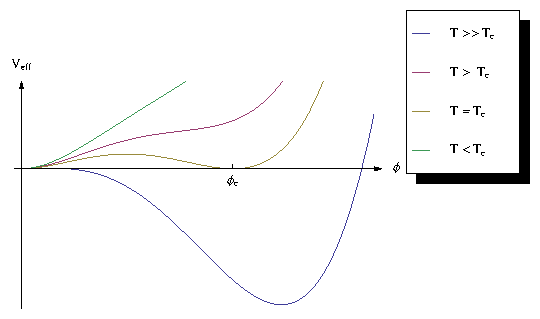
\includegraphics[width=0.7\linewidth]{Images/Higgs}
	\caption{Effective Higgs potential for different temperatures in case of a first order phase transition}
	\label{fig:higgs}
\end{figure}


%%% mode: latex
%%% TeX-master: "../Leptogenesis"
%%% End:
	\chapter{Outline of leptogenesis}
As stated in the section before the SM alone isn't quite enough to describe the observed baryon abundance, so the SM has to be expanded to that effect that it can describe such phenomena. \newline
Although are efforts made to explain direct baryogenesis using GUT theories, there is an much more favored alternative, namely the so called barygenesis via leptogenesis, what this and the following section will be about. 
\section{Expandig the SM}
There are experimental reasons why the SM doesn't tell the whole story about our universe, namely the results of neutrino oscillation experiments. Before the discovery of these neutrino oscillations it was accepted that neutrinos are massless and therefore their left-handedness is well defined. But being able to oscillate between different flavours implies that neutrinos aren't massless and therefore are not purely left-handed and even more so that right-handed neutrinos exist. The easisest way to implement right-handed neutrinos into the SM would be to show, that neutrinos are so-called Majorana particles, which, in contrast to Dirac particles, are their own anti-particles. This would mean that the right-handed neutrinos are right-handed antineutrinos at the same time, but it was already shown that latter exist. Theoretically the way to describe Majorana masses would be to exchange the usual mass term including the Higgs field for a Majorana mass terms, that can be written in the following way \cite[p. 18]{Taanila:2008}, to the SM Lagrangian.
\begin{equation*}
	\mathcal{L}_M=-\frac{1}{2}\overline{\Psi^C}M^M\Psi
	\label{eq:majorana}
\end{equation*}
where the superscript C stands for the charge conjugated neutrino field defined by
\begin{equation*}
	\Psi^C\equiv C\gamma_0\Psi^*
\end{equation*}
with the marix C, which is dependend on the representation of the gamma matrices. The Majorana mass M$^M$ is an n$_F\times$n$_F$ matrix with n$_F$ again the number of particle families. \newline
Using the representation of the U(1)$_Y$ symmetry group given in the previous section, it can easily be seen that in general by using a mass term like in \ref{eq:majorana} to the SM Lagrangian this symmetry is no longer viable.
\begin{equation*}
	\overline{\Psi^C}\Psi \overset{U(1)Y}{\longrightarrow}\overline{(e^{i\frac{Y}{2}\alpha}\Psi)^C}e^{i\frac{Y}{2}\alpha}\Psi=\overline{e^{-i\frac{Y}{2}\alpha}\Psi^C}e^{i\frac{Y}{2}\alpha}\Psi=e^{i\frac{Y}{2}\alpha}\overline{\Psi^C}e^{i\frac{Y}{2}\alpha}\Psi\neq	\overline{\Psi^C}\Psi
\end{equation*}
The relation above shows, that by using Majorana masses of particles with hypercharge Y$\neq$0, like the left-handed neutrinos, one cannot preserve the SM Lagrangians SU(2)$_L\times$U(1)$_Y$ symmetry. 
\newline
That being said right-handed Dirac mass terms for neutrinos have to be added to the Lagrangian in order for it to still preserve its SU(2)$_L\times$U(1)$_Y$ symmetry. Since, like all other right-handed particles in the SM, the right-handed neutrinos form a SU(2)$_Y$ singlet, which we will call N. Also using the isospin conjugate of the Higgs doublet 
\begin{equation*}
	\tilde{\phi}\equiv i\sigma^2\phi^*
\end{equation*}
the Yukawa term can be written as
\begin{equation}
	\mathcal{L}_{\text{N,Yuk}}=h_{ij}\overline{N_i}\tilde{\phi}^\dagger l_j +h_{ij}^* \overline{l_i}\tilde{\phi} N_j
	\label{eq:Yukterm}
\end{equation}
This interaction term will be of analyzed in more detail in Appendix A.1. \newline
The h$_{ij}$ describe the Yukawa couplings and the l$_i$ the left-handed lepton SU(2) doublets of the Standard modell. It can be shown, that this additional term doesn't violate the symmetries of the SM Lagrangian. \newline
However, as explained above adding left-handed Majorana neutrino mass terms to the SM Lagrangian breaks its symmetry, but since right-handed neutrinos have to be added anyways one can also try to add a right-handed Majorana mass term, too.
\begin{equation}
\mathcal{L}_{N,M}=-\frac{1}{2}\overline{N^C}M^MN
\label{eq:neutrino_majorana}
\end{equation}
The mass term in equation \ref{eq:neutrino_majorana} however doesn't violate the Lagrangian's SU(2)$_L\times$U(1)$_Y$ symmetry, because for right-handed neutrinos T=T$^3$=Y=0 and therefore the transformations given in the previous section become the trivial identity transfomation. Anyways, the Dirac Lagrangian, so the SM Langrangian without any Majorana mass terms, is obviously invariant under any U(1) transformation, not only under U(1)$_Y$ transformations. The Majorana mass terms on the other hand are only invariant under the exactly this U(1)$_Y$, especially only for particles with T=T$^3$=Y=0 like the right-handed neutrinos while violating other U(1) symmetries. And according to the Noether theorem, every symmetry of a theory results in a conserved current or quantum number, so breaking the U(1) symmetry not assigned to the hypercharge by using Majorana mass terms one certain quantum number, in this case breaking the following U(1)$_l$ symmetry results in a non-conservation of the lepton number.
\begin{equation}
	\Psi\overset{U(1)_L}{\longrightarrow}e^{i\ell\alpha(x)}\Psi
\end{equation}
with the lepton number $\ell$ of the field $\Psi$.
This seems rather obvious because if Majorana particles are particles and anti-particles at the same time one cannot assing them a distinct lepton number and therefore it is not conserved. \newline
Finally, after putting the Dirac and Majorana mass terms together one ends up with \cite[p. 21]{Taanila:2008}
\begin{equation}
	\mathcal{L}_{M+D}=\left(\overline{\nu^C_L},\overline{N}\right)	\left(\begin{array}{cc}M^M_L&m^D\\m^D&M^M_R\end{array}\right)	\left(\begin{array}{c}\nu_L\\N^C\end{array}\right)+h.c.
	\label{eq_majorana_dirac}
\end{equation}
The matrix m$^D$ contains the masses of the Dirac neutrinos, so the neutrinos found in nature up until now, while M$^M_L$ and M$^M_R$ describe the masses of the left as well as the right-handed Majorana neutrinos. All of these matrices are of the dimension n$_F\times$n$_F$ with n$_F$ the number of neutrino flavours. Also, as explained above, since it isn't possible to introduce left-handed Majorana neutrinos to the SM without violating its fundemental symmetry M$^M_L$ has to be equal to zero.
\section{The seesaw Mechanism}
Although the addition of neutrino masses can be described using the mass term \ref{eq_majorana_dirac} or rather
\begin{equation}
\mathcal{L}_{M+D}=\left(\overline{\nu^C_L},\overline{N}\right)	\left(\begin{array}{cc}0&m^D\\m^D&M^M_R\end{array}\right)	\left(\begin{array}{c}\nu_L\\N^C\end{array}\right)+h.c.
\label{eq_majorana_dirac_zero}
\end{equation}
there is still a problem, namely why the neutrino masses are many orders of magnitude smaller than those of the other SM particles. This however can be described using the so called seesaw mechanism. In this discussion only the so called type I seesaw mechanism will be presented. By doing so the following two assumtions have to be made:
\begin{enumerate}
	\item The Dirac masses arise directly from the Higgs mechanism that gives mass to all SM particles, introducing the electroweak mass scale of order $\sim10^2-10^3$ GeV.
	\item The Majorana masses are much bigger than the Dirac masses, m$^D\ll$ M$^M$. This mass scale arises from GUT's and is of order $\sim10^{10}-10^{16}$ GeV.
\end{enumerate}
The subscript R will be dropped from now on since there is no non-zero left-handed Majorana mass and therefore no further distinction is needed.\newline
Now, after diagonalising the mass matrix in \ref{eq_majorana_dirac_zero} \cite[pp. 2-3]{Lindner:2001hr}, one gets two mass eigenvalues, in particular
\begin{align*}
	M_1&\backsimeq-m^D{\left(M^M\right)}^{-1}{\left(m^D\right)}^{T}\\
	M_2&\backsimeq M^M
\end{align*}
or for just one neutrino family
\begin{align}
	M_1&\backsimeq -\frac{m_D^2}{M^M}
	\label{eq:light_neutrino}
	\\
	M_2&\backsimeq M^M
	\label{eq:heavy_neutrino}
\end{align}
The negative sign for M$_1$ comes from the fact that these are just the eigenvalues of the mass matrix given in \ref{eq_majorana_dirac_zero}, the physical masses are the absolute values of these eigenvalues. \newline
Finding the corresponding eigenstates for each eigenvalue one gets that the eigenstate associated with M$_1$ is $\nu$, the observable, left-handed light neutrino. One can now easily see that the smallness of the neutrino masses compared to those of all the other SM particles comes from the assumption m$^D\ll$ M$^M$. On the other hand however the eigenstate appendant to $M_2$ is N, the newly added, right-handed heavy neutrino, that will play a crucial role in leptogenesis. The heavy neutrino mass being mostly governed by the Majorana mass implies that the right-handed neutrinos are Majorana particles, which means they are their own anti particles.\newline
Interesting to note as well is how these two masses behave under finetuning. It is quite obvious from equation \ref{eq:light_neutrino} that by raising the large mass scale and as a consequence thereof raising the mass of the heavy neutrino the mass of the light neutrinos gets even lower and vice versa, hence the name seesaw mechanism. 
\section{Leptogenesis and the Sakharov conditions}
After the necessary expansion of the SM was performed in the previous section, this section will focus on how the right-handed, heavy neutrinos are able to produce a net, non-zero baryon number, that is how the Sakharov conditions can be fullfilled using this exapanded SM. 
\newline
In the following discussions the assumption that three heavy right-handed neutrinos exist will be made. In addition it is required that the masses of these neutrions are hierarchical in the sense that M$_1\ll$ M$_{2,3}$ and that only the lightest of these neutrinos actually play a significant role for leptogenesis.
\newline
The key ingredient for baryogenesis via leptogenesis is the decay of the heavy, right-handed neutrinos introduced above, that is described by the Yukawa interaction in \ref{eq:Yukterm}.The Feynman diagrams for both decay channels are depicted in figure \ref{fig:N-decay}. The right-handed neutrinos being Majorana particles as a result of the seesaw mechanism they don't preserve lepton number and because of this they can decay into leptons as well as anti leptons, as it can be seen in figure \ref{fig:N-decay}.
\begin{figure}[H]
	\begin{equation*}
	\feynmandiagram [baseline=(d.base), horizontal=d to b] {
		b -- [scalar, edge label=\(\overline{\phi}\)] a,
		b-- [fermion, edge label =\(\ell\)] c,
		d   -- [edge label=N] b}; 
	\qquad \text{or} \qquad
	\feynmandiagram [baseline=(d.base), horizontal=d to b] {
		b -- [scalar, edge label = \(\phi\)] a,
		b-- [anti fermion, edge label=\(\overline{\ell}\)] c,
		d  --[edge label=N] b  }; 
	\end{equation*}
	\caption{Feynman diagrams for the N-decay}
	\label{fig:N-decay}
\end{figure}
\subsubsection{B violation}
The B violation in the frame of leptogenesis is achieved in the same way as in direct electorweak baryogenesis via the B+L violating sphaleron processes. Because of the eventually by N decays produced net lepton number this means that the lepton abundance is converted into a baryon abundance by these processes.
\subsubsection{C and CP violation}
As in direct baryogenesis C violation is already maximally violated SM electroweak interaction, so this is also the case in this slightly extended model.
The CP violation for the N$_1$ decay however is a bit more complicated, since for it to be calculated one has to take the one-loop Feynman diagrams additional to the tree level decay into account. The interference between these diagramms gives than rise to the CP violation needed for successfull baryogenesis. These one-loop diagrams are depicted in figure \ref{fig:N_loop}.
\begin{figure}[H]
	\begin{equation*}
	\feynmandiagram [baseline=(d.base), horizontal=a to t1] 
	{
		
		a  -- [edge label=\(N_i\)] t1 --[anti fermion,edge label=\(\ell\)] t2 --[edge label=\(N_j\)] t3 -- [scalar,edge label=\(\phi\)]t1, t2 -- [scalar, edge label=\(\phi\)] p2,
		t3 -- [fermion, edge label=\(\ell\)] p1 ,
		
	};
	\qquad +\qquad
	\feynmandiagram [baseline=(d.base), horizontal=b to c] 
	{ 
		a --[edge label =\(N_i\)]b
			-- [half left, looseness=1.5, edge label = \(\ell\text{,}\overline{\ell}\)] c
			-- [scalar, half left, looseness=1.5,edge label = \(\phi\)] b, 
		c -- [edge label = \(N_j\)]d --[scalar, edge label =\(\phi\)] e,
		d--[fermion, edge label =\(\ell\)]f
	
	};
	\end{equation*}
	\caption{One-loop diagrams for the N-decay}
	\label{fig:N_loop}
\end{figure}
\noindent
By comparing this figure to \cite[Fig. 5.1]{Davidson:2008bu} one sees that in figure \ref{fig:N_loop} one diagramm is missing. This missing diagram hoever doesn't contribute to the CP violation and therefore it was neglected. The distinction between N\textsubscript{i} and N\textsubscript{j} has to be made since the virtual neutrinos trasmissioned during these processes aren't of the same flavour as the neutrino in the initial state. This means that in order for CP to be violated there has to exist at least an extra neutrino next to the lightest one. \newline
This being said one can calculate the CP asymmetry\cite[pp. 24ff.]{Davidson:2008bu}, which is in general defined as
\begin{equation}
	\epsilon=\frac{\Gamma(N_1\rightarrow\overline{\phi}\ell)-\Gamma(N_1\rightarrow\phi\overline{\ell})}{\Gamma(N_1\rightarrow\overline{\phi}\ell)+\Gamma(N_1\rightarrow\phi\overline{\ell})}
	\label{eq:CP_violation}
\end{equation}
by interfering the tree level decay with the one-loop decays. This results in \cite[p. 26]{Davidson:2008bu}
\begin{equation}
	\epsilon\gtrsim10^{-6}
	\label{eq:CP_value}
\end{equation}
Although this value is rather small it isn't zero and therefore the CP symmetry is violated by the decay of heavy right-handed Majorana neutrinos. 
\subsubsection{Deviation from the equilibrium}
The last condition that has to be met for successfull baryogenesis is that the decay of the heavy neutrinos must occur outside of equilibrium. For high enough temperatures, namely for T $\gtrsim$ M\textsubscript{1}, the decay of the neutrino is in equilibrium with the inverse decay $\phi\ell\rightarrow N$ and no net lepton number can be produced even if the other two conditions hold as shown in sec. 2.1.2. Even if during inflation an abundance of N was produced the lepton asymmetry would washed out by equilibrium processes as soon as the temperature rises up to at least the mass of the heavy neutrino during the reheating phase of the ealrly universe. \newline
However if the temperature drops below M$_1$ the heavy neutrino inverse decay is exponentially surpressed by a Boltzmann factor because with falling temperature it becomes exponentially more unprobable for a lepton and Higgs to have enough energy to form a heavy neutrino, while the neutrinos themselves can still decay into lepton and Higgs. Because of this the equilibrium density of the neutrinos is also heavily Boltzmann surpressed and if the decay rate is small enough the actual neutrino density can be greater than the equilibrium density and stay greater for an considerable amount of time. This means that decays happening before the actual neutrino density converges to the equilibrium density actually happen outside of equilibrium and a net lepton number can be produced that, because of surpression of inverse decays, won't be washed out and as a consequence thereof will be transformed into a baryon abundance through the B+L violating electroweak sphaleron processes, that will still be active as the heavy neutrino mass at least of order of the upper limit of the temperature range in which sphaleron processes act. \newline
The requirement for the neutrino decay to be slow enough to sustain its out-of-equilibrium state is the following \cite[p. 30]{Taanila:2008}.
\begin{equation}
	\Gamma_D<H
	\label{eq:out_of_eq}
\end{equation}
$\Gamma_D$ denotes the total decay rate of the neutrinos while H is the expansion rate of the universe. This relation is equivalent to the one given in \ref{eq:rate_s_hubble} as a requirement for processes to be out of equilibrium. 
	 \chapter{Analytic approximations and calculations}
\section{Rate equations for leptogenesis}
Now in order to qualitatively describe leptogenesis one has to consider rate equations for the lepton number and B-L number densities. In a static universe without lepton number violating processes the rate equation would trivialy be
\begin{equation}
	\frac{d}{dt}n=0
	\label{eq:rate_static_nointeraction}
\end{equation}
If one now condsiders a universere expandig with the rate H the rate equation above changes to.
\begin{equation}
\left(\frac{d}{dt}+3H\right)n=0
\label{eq:rate_expanding_nointeraction}
\end{equation}
Finally including lepton number violating processes the rate equation one obtains for the neutrino number density is
\begin{equation}
\left(\frac{d}{dt}+3H\right)n_N=-\Gamma_N\left(n_N-n_N^{eq}\right)+\Gamma_{N,B-L}n_{B-L}
\label{eq:L_rate_expanding_interaction}
\end{equation}
Applying this reasoning to the B-L number density yields
\begin{equation}
\left(\frac{d}{dt}+3H\right)n_{B_L}=\Gamma_{B-L,N}\left(n_N-n_N^{eq}\right)+\Gamma_{B-L}n_{B-L}
\label{eq:B-L_rate_expanding_interaction}
\end{equation}
The coefficient $\Gamma_N$ denotes how fast the neutrino density equalizes with its equilibrium density, while $\Gamma_{B-L}$ describes the washout of a net B-L number. $\Gamma_{B-L,N}$ describes how the B-L asymmetry is affected by the deviation of the neutrino density from its equilibrium value and together with $\Gamma_{N,B-L}$ these two coefficients characterize CP violating processes \cite[p. 4]{Bodeker:2013qaa}. Since both these coefficients describe CP violating processes they must depend on the CP violating parameter $\epsilon$ introduced in the section before and it was also seen there that this parameter is small vor heavy neutrino decays and therefore the second term in equation can be neglegted. \newline
The goal now is to determine these coefficients at least at leading order and the first one will be $\Gamma_N$. To get this coefficient one has to integrate equation \ref{eq:L_rate_expanding_interaction} over phase space, resulting in
\begin{equation}
	\left(\frac{\partial}{\partial t}-Hp\frac{\partial}{\partial p}\right)f_N=\Gamma_N\left(e^{E_N/T}-f_N\right)
	\label{eq:boltzmann}
\end{equation}
The whole calculation on how performing the phase space integral can be found in appendix \ref{ap:phase_space}. \newline
One might now notice that equation \ref{eq:boltzmann} differs from equation 4 in \cite{Bodeker:2013qaa} by a factor of $\frac{M_N}{E_N}$, that origins in a different normaliziation of the phase space. However, since we operate in a non-relativistic regime E\textsubscript{N} $\approx$ M\textsubscript{N} and therefore this factor is $\sim$ 1 and negligible. Using this argumentation one can also see that $\Gamma_N=\Gamma_0$ with $\Gamma_0$ the total decay rate of the heavy neutrinos, wich is governed by the Yukawa interaction term \ref{eq:Yukterm}. It has to be mentioined that for the equilibrium distribution the Boltzmann statistic with neglegted chemical potential was used since the energy of a neutrino E\textsubscript{N} $\approx$ M\textsubscript{N} $\gg$ T during the phase where the decay happen outside equilibrium and therefore quantum mechanical effects play an insignificant role and can be neglected. Going back to the decay rate, that can be calculated as done in appendix \ref{ap:tree_level_decay}, one gets
\begin{equation}
\Gamma_N=\Gamma_0=\frac{|h_{11}|^2M_N}{8\pi}
\label{eq:Gamma_N}
\end{equation}
\todo{Gamma B-L,N erklären}
Since the coefficient $\Gamma_{B-L}$ refers to the washout of the B-L asymmetry it arises from the inverse decay l$\phi\rightarrow$ N and can be calculated via \todo{Integralherleitung klären}
\begin{equation}
\Gamma_{B-L}n_{B-L}=\int\prod_{a=N,\ell,\phi}\frac{d^3p_a}{2E_a(2\pi)^3}(2\pi^4)\delta(p_\ell+p_\phi-p_N)(	f_\ell f_\phi-f_{\bar{\ell}}f_{\bar{\phi}})\sum|M_0|^2
\label{eq:Gamma_B-L}
\end{equation}
$\sum|M_0|^2=16\pi M_N\Gamma_0$ describes the tree level matrix element for exactly this inverse decay summed over all spins of N and isospin components of $\ell$. In order to evaluate this integral properly one has to first describe the term $(	f_lf_\phi-f_{\bar{l}}f_{\bar{\phi}})$ more precisely. Since we operate at rather hight temperatures one can use Boltzmann statistics for lepton and Higgs regardless and expanding in the chemical potentials up to first order yields.
\begin{equation}
	f_\ell f_\phi-f_{\bar{\ell}}f_{\bar{\phi}}\simeq 2e^{-\frac{E_N}{T}}\frac{\mu_l+\mu_\phi}{T}
	\label{eq:distri_diff}
\end{equation}
As mentioned in \cite[p. 7]{Bodeker:2013qaa} the chemical potentials are proportional to the B-L number density and by using the coefficients c$_l$ and $c_\phi$ in order to avoid introducing the exact temperature dependend relations one can also connect n$_{B-L}$ to the lepton and Higgs asymmetries through \cite[p. 7]{Bodeker:2013qaa}
\begin{align}
	n_\ell-n_{\bar{\ell}}=-c_\ell n_{B-L}
	\label{eq:l-lbar} \\
	n_\phi-n_{\bar{\phi}}=-c_\phi n_{B-L}
	\label{eq:phi-phibar}
\end{align}
Now by expanding the number distribution for leptons and Higgs and their respective anti particles in the chemical potentials up to first order one can finally put the chemical potential and n$_{B-L}$ in relation to each other. It is important to note that one has to use the Fermi-Dirac- and Bose-Einstein distribution for leptons and Higgses respectively. The reason for this is that these two particle species are in equilibrium at the temperature T. Because of this and the fact that they are relativistic particles, their kinetic energy and therefore momenta are of order T and quantum effects can't be neglected. On the other hand it is possible to use Boltzmann statistics for leptons and Higgs bosons above since particles taking part in the production of a heavy neutrions having energies or momenta of order $\frac{M\textsubscript{N}}{2}\gg T$ and quantum effects can safely be neglected in this case. Finally using quantum statistics results in
\begin{align}
\mu_\ell=\frac{3c_l}{T^2}n_{B-L}
\label{eq:chempot_l}
\\
\mu_\phi=\frac{3c_l}{2T^2}n_{B-L}
\label{eq:chempot_phi}
\end{align}
Using all these results and putting them into relation \ref{ap:Gamma_B-L} one gets the following result for the washout rate $\Gamma$\textsubscript{B-L}
\begin{equation}
	\Gamma\textsubscript{B-L}=\frac{3}{\pi^2}\:\left(c_\ell+\frac{c_\phi}{2}\right)z^2K_1(z)\Gamma_0
	\label{eq:Gamma_B-l_result}
\end{equation}
with K\textsubscript{1}(z) the modified Bessel funktion of the second kind and 
\begin{equation}
	z\equiv\frac{M_N}{T}
\end{equation}
what can be seen as an unitless measure for time, since the temperature of the universe decreases over time and therefore z increases. 
The exact derivation of these results can be looked up in appendix \ref{ap:Gamma_B-L}. \newline
Using the relations given in \ref{eq:rate_g_hubble} and \ref{eq:rate_s_hubble} it is usefull to define the so called wash out factor K as follows
\begin{equation}
	K\equiv\left.\frac{\Gamma_0}{H}\right|_{T=M\textsubscript{N}}
\end{equation}
Using this and equation 3 of \cite{Buchmuller:2004nz}
\begin{equation}
	H(z)=\left.H\right|\textsubscript{T=M\textsubscript{N}}\cdot \frac{1}{z^2}
	\label{eq:H_von_z}
\end{equation}
one can now compare the rates calculated above to the Hubble constant H.\newline
For T $\lesssim$ M\textsubscript{N} one can approximate $\Gamma\textsubscript{N}$ as $\Gamma_0$ what results in 
\begin{equation}
	\frac{\Gamma_\textsubscript{N}}{H}\simeq\frac{\Gamma_0}{\frac{1}{z^2}\left.H\right|\textsubscript{T=M\textsubscript{N}}}=z^2K
	\label{eq:Gamma_N_H}
\end{equation}
Since z increases with time, equation \ref{eq:Gamma_N_H} clearly shows that the rate with which the neutrino number density approaches its equilibrium value gets more and more greater than the expansion of the universe and therefore the deviation from equilibrium vanishes over time. \newline
Looking at \ref{eq:Gamma_B-l_result} one can easily see that for T $\sim$ M\textsubscript{N}, or z $\approx$ 1, $\Gamma\textsubscript{B-L}$ is of the same order as $\Gamma\textsubscript{N}$, since K$_1$(1)=$\mathcal{O}$(1). On the other hand however for really low temperatures, so T $\ll$ M\textsubscript{arg} or z very big, one can see the quantitative behaviour of $\Gamma\textsubscript{B-L}$ by using the asymptotic expansion of the modified Bessel function given by
\begin{equation*}
	K\textsubscript{n}(z)\sim\sqrt{\frac{\pi}{2z}}e^{-z}\sum_{k=0}^{\infty}\frac{a\textsubscript{k}(n)}{z^k}
\end{equation*}
with a\textsubscript{k}(n) some coefficients that don't are of any interest for this matter. Now using this and dropping all but the first term of the sum above, what is justified because z is so big, one gets
\begin{equation}
	\frac{\Gamma\textsubscript{B-L}}{H}\sim\sqrt{\frac{1}{z}}e^{-z}z^2\frac{\Gamma_0}{\frac{1}{z^2}\left.H\right|\textsubscript{T=M\textsubscript{N}}}=z^\frac{7}{2}e^{-z}K
	\label{eq:Gamma_B-L_H}
\end{equation}
So because $\Gamma\textsubscript{N}$ increases with z for z $\approx$ 1 so does $\Gamma\textsubscript{B-L}$. However as equation \ref{eq:Gamma_B-l_result} suggests, $\Gamma\textsubscript{B-L}$ gets more and more suppressed by the exponential factor for increasing z and therefore has to have some maximum. Additionally for sufficiently low temperatures, like the extremely low 2.7 K of the present universe, the washouth rate $\Gamma\textsubscript{B-L}$ is effectively zero and any symmetry produced in earlier times is frozen out. 
All this can be seen in figure \ref{fig:rates} where the previously calculated ratios are plotted against z and are normalized to the washout factor K.
\begin{figure}[H]
	\centering
	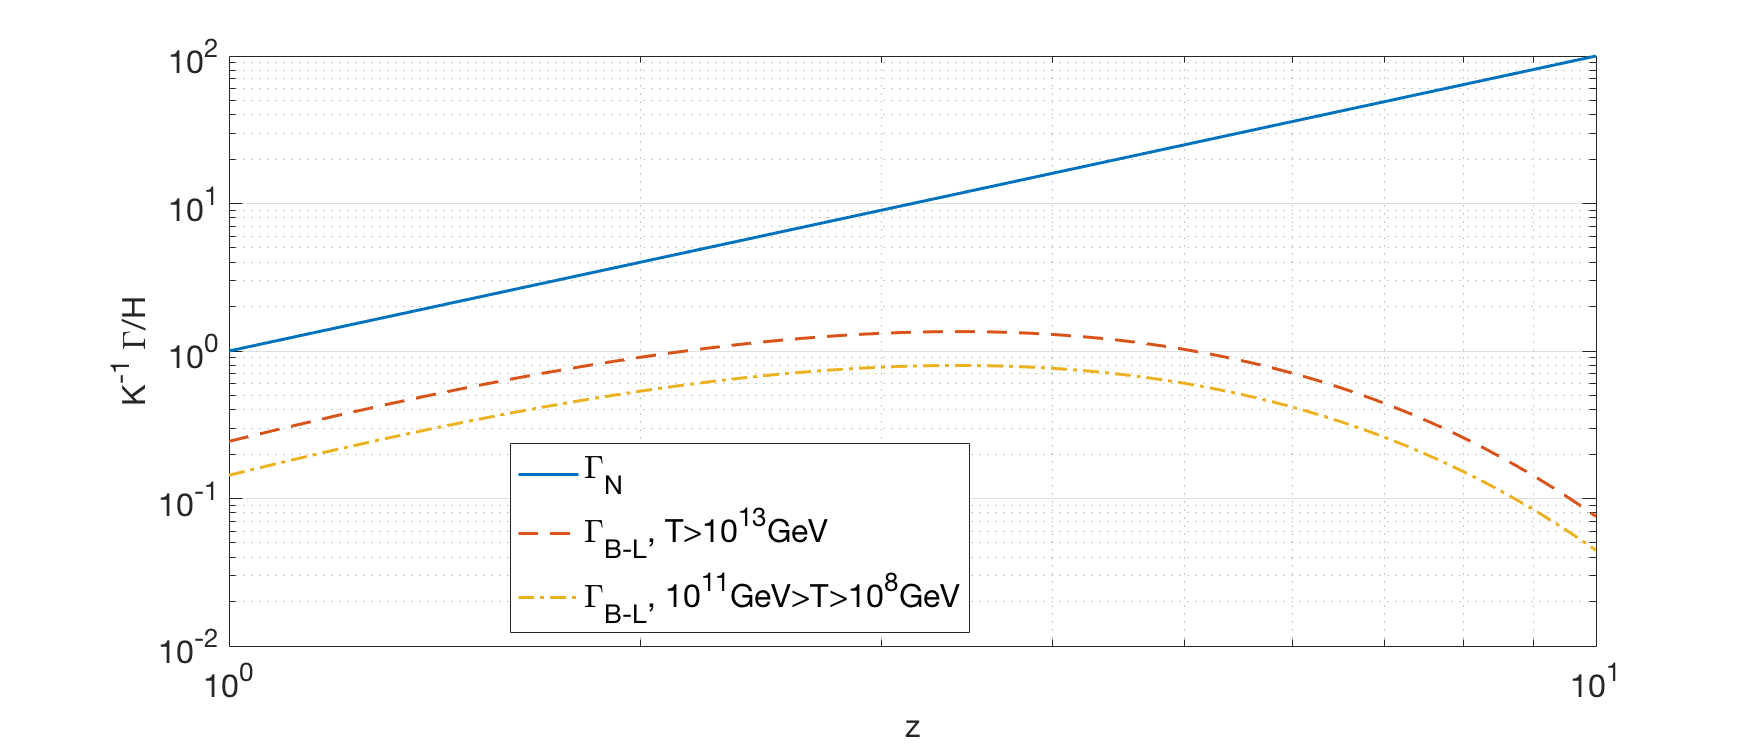
\includegraphics[width=0.8\linewidth]{Images/rates}
	\caption{The ratios $\Gamma\textsubscript{N}$/H and $\Gamma\textsubscript{B-L}$/H plotted against H}
	\label{fig:rates}
\end{figure}
\section{Relativistic corections}
\section{Radiative corrections}
	\chapter{Numerical results} \label{sec:num_results}
In order to quantify the results of the previous chapter, it is usefull to parameterize the solutions of the rate equations above, especially the solution for the $B-L$ asymmetry described by \eqref{eq:B-L_rate_expanding_interaction} or \eqref{eq:B-L_rate_expanding_interaction_rel} using the so called final efficiency factor $\kappa_f$ defined via
\begin{equation}
\lim\limits_{z\rightarrow\infty}\frac{n_{B-L}}{n_\gamma^{eq}}=\frac{3}{4}\epsilon\kappa_f,
\label{eq:final_efficiency}
\end{equation}
with $n_\gamma^{eq}=2\zeta(3)T^3/\pi^2$ the equilibrium density of photons and $\epsilon$ the CP-asymmetry parameter. It is now more convenient to rewrite the rate equations in terms of
\begin{equation}
	X_i\equiv\frac{n_i}{T^3},
	\label{eq:X_i}
\end{equation}
 with $i=B-L,N$. Using this substitution, one has to consider the transformation \cite[Eq. 7.1]{Wormann:2016yyi}
\begin{equation}
\frac{d}{dt}(X_iT^3)+3Hn_i=\frac{dX_i}{dt}T^3.
\end{equation}
Also, since the limit in \eqref{eq:final_efficiency} considers $z$ instead of the time $t$ one has to change the dependence from $t$ to $z$ by using
\begin{equation}
\frac{d}{dt}=\frac{dz}{dt}\frac{d}{dz}=\frac{dz}{dT}\frac{dT}{dt}\frac{d}{dz}=-\frac{M_N}{T^2}(-HT)\frac{d}{dz}=zH\frac{d}{dz},
\end{equation}
where the relation $dT/dt=-HT$ \cite[p. 3]{HahnWoernle:2009qn} was used. \newline\indent
Combining all these results in the new, uncorrected rate equations gives
\begin{equation*}
zH\frac{dX_N}{dz}=-\Gamma_0\left(X_N-X_N^{eq}\right),
\end{equation*}
\begin{equation*}
zH\frac{dX_{B-L}}{dz}=\Gamma_0\left[\epsilon\left(X_N-X_N^{eq}\right)-\frac{3}{\pi^2}\:\left(c_\ell+\frac{c_\phi}{2}\right)z^2K_1(z)X_{B-L}\right],
\end{equation*}
Now by dividing these rate equations by the factor $zH$ and by using \eqref{eq:washout} one finally arrives at
\begin{equation}
\frac{dX_N}{dz}=-zK\left(X_N-X_N^{eq}\right),
\end{equation}
\begin{equation}
\frac{dX_{B-L}}{dz}=zK\left[\epsilon\left(X_N-X_N^{eq}\right)-\frac{3}{\pi^2}\:\left(c_\ell+\frac{c_\phi}{2}\right)z^2K_1(z)X_{B-L}\right].
\label{eq:X_B-L}
\end{equation}
To be able to relate the result of these rate equations it is useful to express equation \eqref{eq:X_B-L} in terms of
\begin{equation}
	N_{B-L}\equiv\frac{n_{B-L}}{n_\gamma^{eq}}=\frac{\pi^2}{2\zeta(3)}X_{B-L},
\end{equation}
yielding
\begin{equation}
\frac{dN_{B-L}}{dz}=\frac{\pi^2}{2\zeta(3)}\epsilon zK\left(X_N-X_N^{eq}\right)-\frac{3}{\pi^2}\:\left(c_\ell+\frac{c_\phi}{2}\right)z^3K_1(z)KN_{B-L}.
\label{eq:N_B-L}
\end{equation}
Now, in order to finally remove the last unkown parameter in \eqref{eq:N_B-L}, namely the CP-asymmetry parameter $\epsilon$ one can use the efficiency factor $\kappa(z)$, which is, analogously to \eqref{eq:final_efficiency}, defined via
\begin{equation}
	\frac{n_{B-L}}{n_\gamma^{eq}}=\frac{3}{4}\epsilon\kappa,
	\label{eq:efficiency}
\end{equation} 
where $\kappa(\infty)=\kappa_f$,to rewrite equation \eqref{eq:N_B-L} resulting in
\begin{equation}
\frac{d\kappa}{dz}=\frac{2\pi^2}{3\zeta(3)}zK\left(X_N-X_N^{eq}\right)-\frac{3}{\pi^2}\:\left(c_\ell+\frac{c_\phi}{2}\right)z^3K_1(z)K\kappa.
\label{eq:kappa}
\end{equation}
The next step will be to introduce the relativistic corrections to these rate equations. For this they have to be normalized in a similar but different way as the one in equation \eqref{eq:X_i}\cite[Eq. (7.9)]{Wormann:2016yyi}:
\begin{equation}
	X_u\equiv\frac{M_N^2}{T^5}u=\frac{z^2}{T^3}u,
	\label{eq:X_u}
\end{equation}
with $u$ given in \eqref{eq:energy_density}.\newline \indent
Substituting this for $u$ in the equations \eqref{eq:L_rate_expanding_interaction_rel}, \eqref{eq:rate_u} and \eqref{eq:B-L_rate_expanding_interaction_rel} and rewriting the rate equations according to the steps above results in\cite[p. 47]{Wormann:2016yyi}
\begin{equation}
\frac{dX_u}{dz}=-zK\left(X_u-X_u^{eq}\right),
\end{equation}
\begin{equation}
\frac{dX_N}{dz}=-zK\left(X_N-X_N^{eq}\right)+\frac{K}{z}\left(X_u-X_u^{eq}\right),
\end{equation}
\begin{equation}
\frac{d\kappa}{dz}=\frac{2\pi^2}{3\zeta(3)}zK\left[\left(X_N-X_N^{eq}\right)-\frac{1}{z^2}\left(X_u-X_u^{eq}\right)\right]-\frac{3}{\pi^2}\:\left(c_\ell+\frac{c_\phi}{2}\right)z^3K_1(z)K\kappa.
\end{equation}
The last thing needed to solve these equations are the two equlibrium distributions $X_N^{eq}$ and $X_u^{eq}$, which are given as
\begin{align}
	X_N^{eq}=\frac{1}{\pi^2}z^2K_2(z),\\
	X_u^{eq}=\frac{3}{2\pi^2}z^3K_3(z).
\end{align}
Their calculation can be looked up in appendix \ref{ap:equlibrium}.\newline \indent
Now, after everything needed to solve the rate equation is available, they were solved using the MATLAB code that can be looked up in appendix \ref{ap:matlab}. The solution starts at $z=1$, since there $p\sim M_N$ and therefore the non-relativistic expansion cannot be used for smaller $z$ \cite[p. 13]{Bodeker:2013qaa}. Also, next to $\kappa(1)=0$, two sets of initial conditions were used for $n_N$ and $u$ or $X_N$ and $X_u$ respectively, the first one being vanishing $X_N$ and $X_u$ while the second set of initial conditions are thermal ones, thermal meaning that the densities $n_N$ and $u$ start at their corresponding equilibrium values for $z=1$. Latter is the more physical and realistic scenario because for $K\gtrsim1$ a reasonable number of right-handed neutrinos will have been produced at $z=1$\cite[p. 13]{Bodeker:2013qaa}. \newline\indent
Figure \ref{fig:efficiency} shows the final efficiency factor plotted against the washout parameter $K$ with and without the relativistic corrections for vanishing und thermal initial conditions, respetively, for a temperature ranging from $10^{8}-10^{11}$GeV. It is easy to see that for small $K\lesssim$ 4 the non-relativistic approximation is not viable because for both sets of intial conditions respectively the results of the non-relativistic and the relativistic calculation differ significantly, with the greatest discrepancy appearing for vanishing initial conditions. On the other hand for $K\gtrsim$ 5 the differences between initial conditions as well as between non-relativistic and relativistic calculation disappear until the four curves run together for $K\sim$ 7. This clearly shows that for a sufficiently high washout parameter the non-relativistic approximation is a feasible way of describing the evolution of the $B-L$ asymmetry and that higher orders of relativistic corrections are not necessary to be included.
\begin{figure}[H]
	\centering
	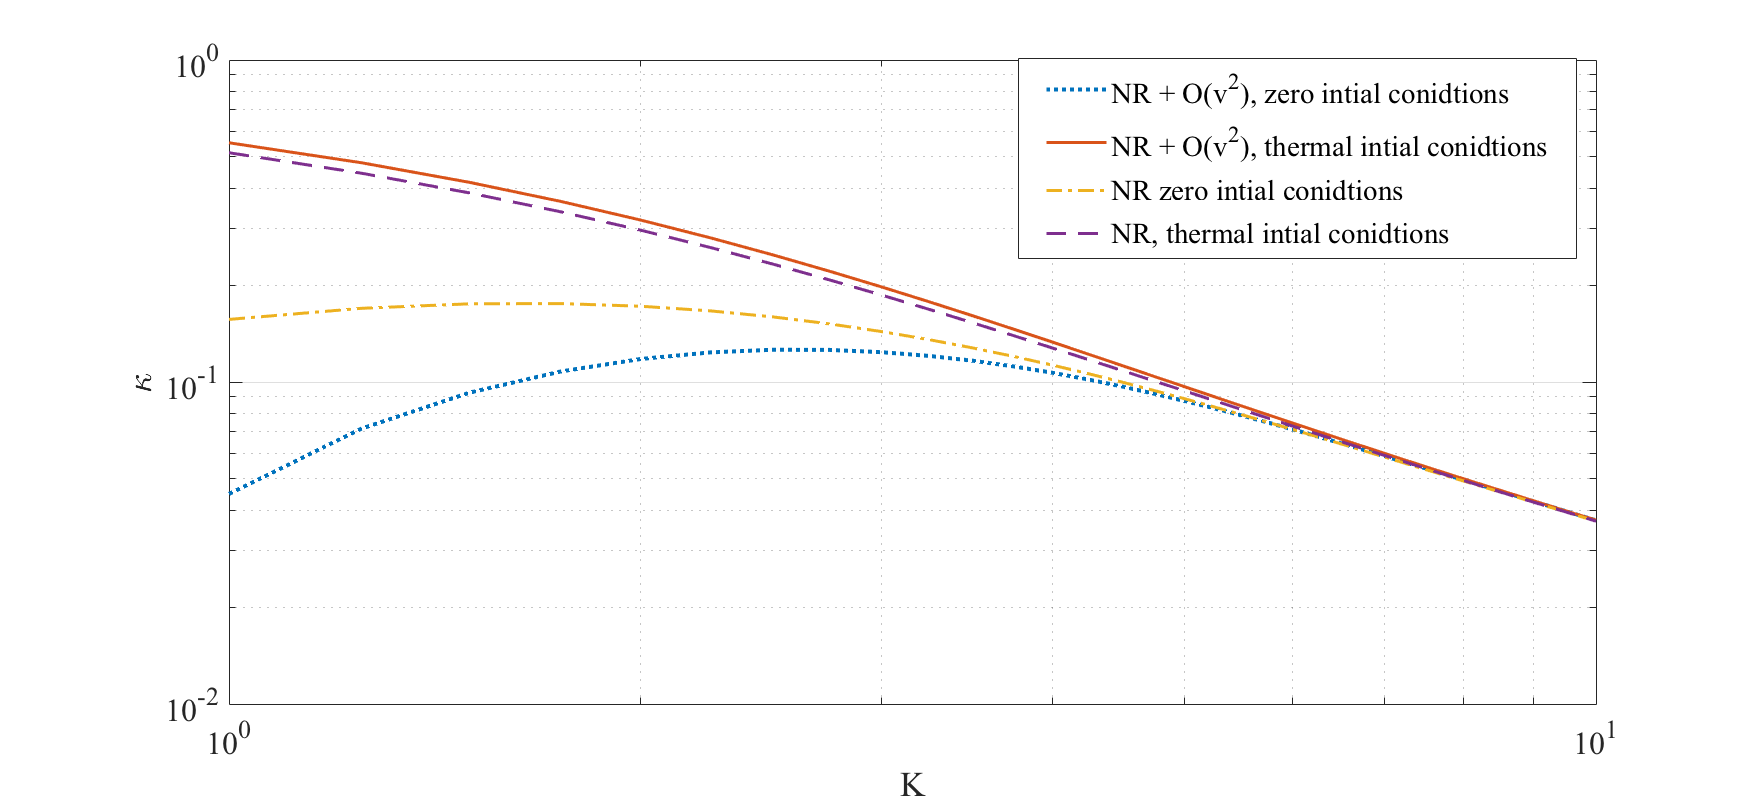
\includegraphics[width=\linewidth]{Images/efficiency}
	\caption{The final efficiency factor depending on the washout strength. The non-relativistic approximation as well as the relativistic corrections are plotted for both zero and thermal initial conditions.The temperature is in a range of $T=10^{8}-10^{11}$GeV.}
	\label{fig:efficiency}
\end{figure}
The next interesting thing to analyze is how the discrepancies between the non-relativistic approximation and the calculation containing $\mathcal{O}(p^2)$ corrrections evolve with growing $K$. This is depicted in figure \ref{fig:corrections}, where relative difference of these two results is plotted against $K$ for different temperature ranges, while thermal intial conditions were used. For small washout parameters clear differences for the different temperature ranges can be seen, however, even for the highest temperatures of $T>10^{13}$ GeV this relative difference merely surpasses 10\%. This differences then drop rapidly for every temperature until they slowly converge for $K\gtrsim10$, where the relative error is already well below 1\%. For even larger $K$, namely $K\sim20$ the relative size of the relativistic corrections is about 0.1\% for every shown temperature range. This again, clearly shows, that for a high enough washout parameter $K$ the non-relativistic approach is perfectly viable. \newline \indent
Now figure \ref{fig:corrections} can be used to analyze \ref{fig:efficiency} in more detail. As mentioned above the 4 curves in \ref{fig:efficiency} run together for $K\sim$ 7 and indeed, by looking at the green, dotted curve in \ref{fig:corrections}, the relative size of the relativistic corrections is about 1.5\% and at the endpoint of \ref{fig:efficiency} at $K=10$ it is 0.7\% and therefore the discrepancy is already below 1\%.
\begin{figure}[H]
	\centering
	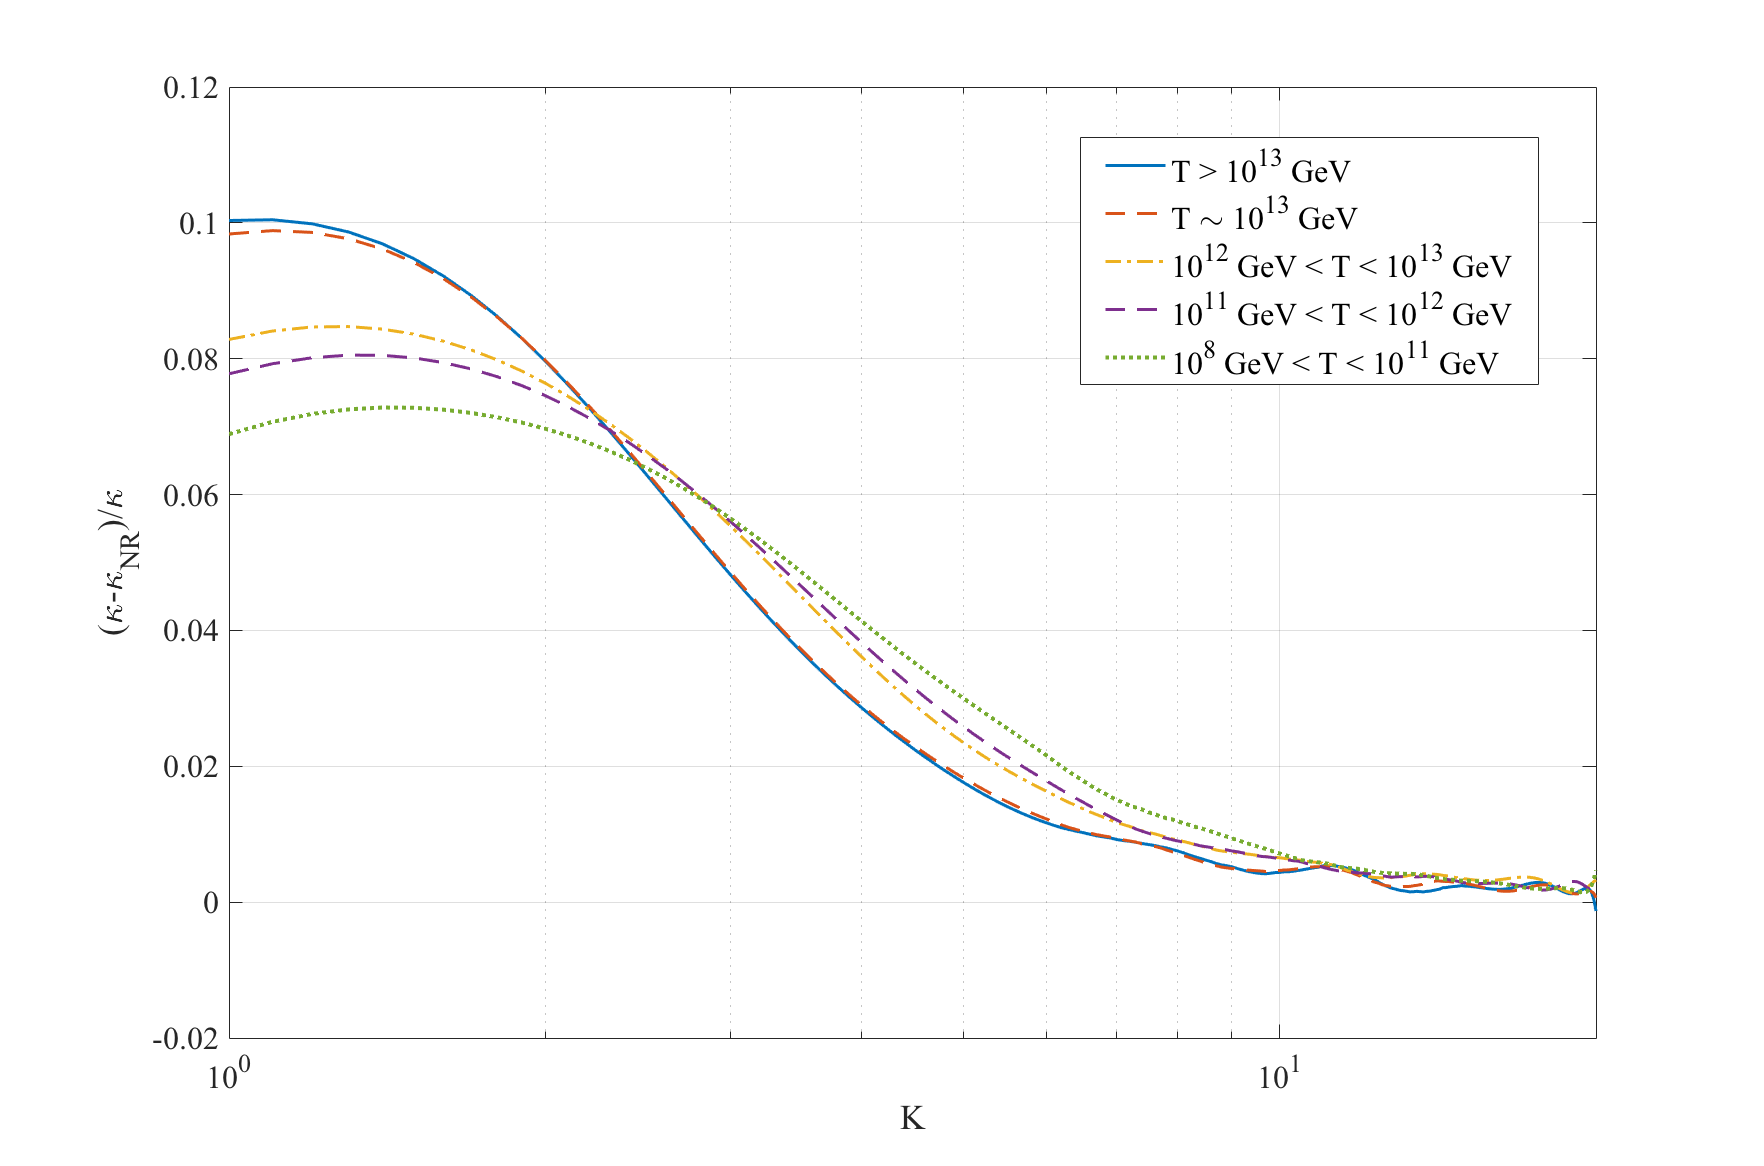
\includegraphics[width=\linewidth]{Images/corrections}
	\caption{The difference of the non-relativistic approximation and the expansion containing the relativistic corrections normalized to the relativistic solution plotted against the washout parameter for different temperature ranges, corresponding to different values of $c_\ell$ and $c_\phi$. Here thermal initial conditions were used.}
	\label{fig:corrections}
\end{figure}
Finally the effect of using the correct quantum statistics over classical Boltzmann statistics and vice versa will be studied and examined. 
During the calculations of the coefficients in the rate equations, more precisely during the calculation of $\Gamma_{B-L}$ there were two occasions in which the explicit forms of particle distributions had to be used, namely for obtaining the equations \eqref{eq:chempot_l} and \eqref{eq:chempot_phi} and even before that for calculating the product $f_\ell f_\phi$. \newline \indent
In the first case quantum statistics were used for leptons and Higgses respectively, yielding the result given in that section. If one uses classical Boltzmann statistics the result changes by a seemingly not that impactful numerical coefficient of 12/$\pi^2$, yielding
\begin{equation}
\Gamma_{B-L}=\frac{1}{4}\:\left(c_\ell+\frac{c_\phi}{2}\right)z^2K_1(z)\Gamma_0,
\label{eq:Gamma_B-l_classical}
\end{equation}
as given in appendix \ref{ap:statistics}.
\begin{figure}[H]
	\centering
	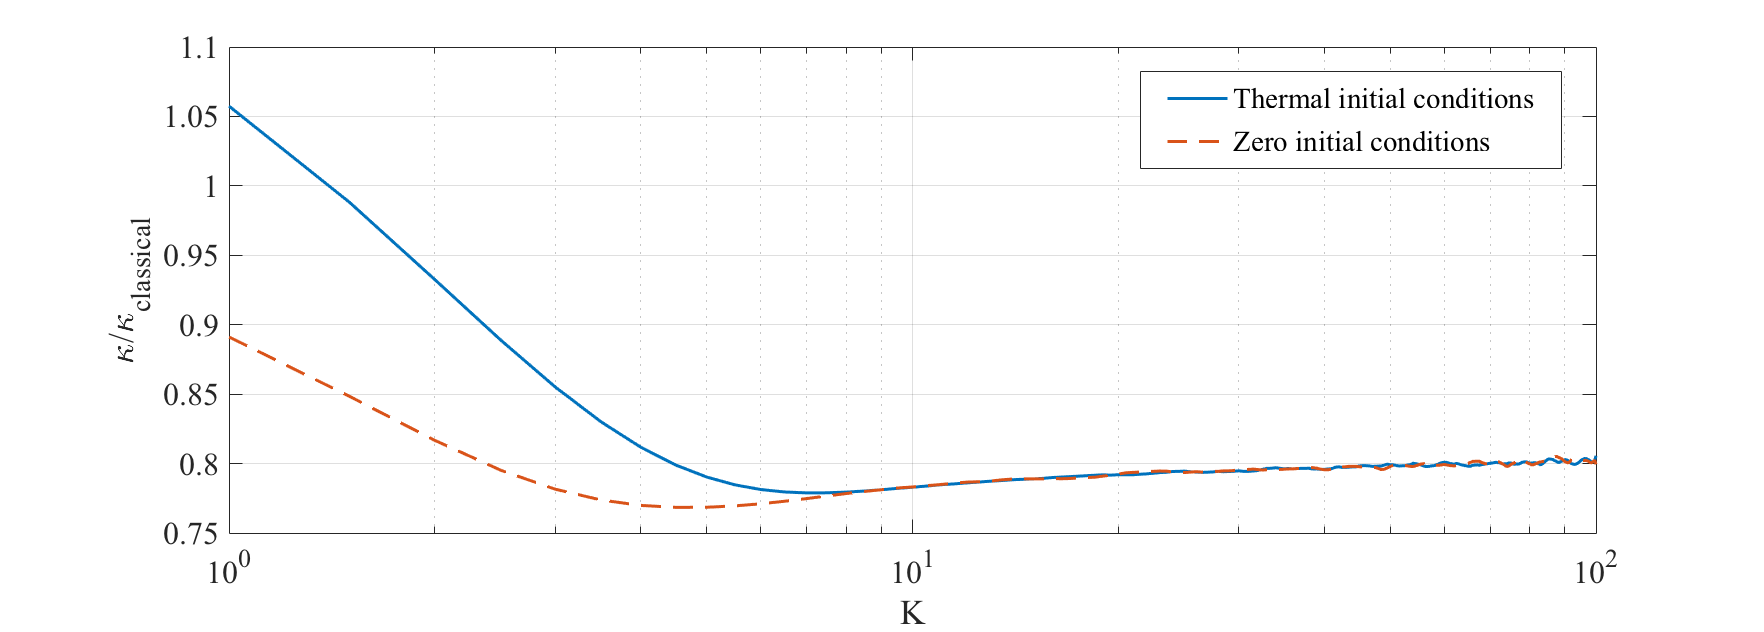
\includegraphics[width=\linewidth]{Images/quantum}
	\caption{The final efficiency factor determined using the respective quantum stastics to obtain equations for the chemical potentials of leptons and Higgses normalized by the final efficiency factor obtained by using classical Boltzmann statistics for thermal and vanishing initial conditions. $c_\ell=1$ and $c_\phi=0$ were used.}
	\label{fig:quantum}
\end{figure} \noindent
Figure \ref{fig:quantum}, however, clearly shows that using Boltzmann statistics drastically changes the final efficiency factor. For small $K$ and thermal initial conditions the classical approximation is about 5\% smaller than the result obtained using quantum statistics, while for zero initial conditions the classical approximation exeeds the quantum calculation by $\sim$11\%. For growing $K$ the classical approximation grows larger, surpassing the quantum calculation more and more and the deviation peaks at about 24\% for $K\simeq$ 5 and zero initial conditions and at about 22\% for $K\simeq$ 7 and thermal initial conditions, respectively. For an even larger washout parameter this deviation slightly lowers until it reaches around 20\% for $K\simeq$ 30 for both sets of initial conditions. From this point on $\kappa/\kappa_{classical}$ practically stays constant for growing $K$.
This clearly highlights the importance of using the right statistics, as using classical statistics is a somewhat good approximation only for small washout parameters, while it completly fails for higher washout parameters.\newline \indent
On the other hand, because the Higgs particles and leptons are of high energy and the corresponding integrals don't saturate at momenta of order $T$ they can be treated using Maxwell-Boltzmann statistics, in order to calculate the quantity $f_\ell f_\phi-f_{\bar{\ell}}f_{\bar{\phi}}$. Nevertheless, it is interesting to see how using the correct quantum statistics and therefore not neglecting their quantum characteristics, affects previous results.
As also shown in appendix \ref{ap:statistics}, this leads the following correction of the coefficient $\Gamma_{B-L}$
\begin{equation}
\Gamma_{B-L}=\frac{3}{\pi^2}\:z^3\left(\frac{e^{z/2}}{e^{z/2}-1}\:\frac{c_\phi}{2}+\frac{e^{z/2}}{e^{z/2}-1}c_\ell\right)\int_{1}^{\infty}dx\frac{\sqrt{x^2-1}}{e^{zx}-1}\Gamma_0.
\label{eq:B-L_corrected}
\end{equation}
\begin{figure}[H]
	\centering
	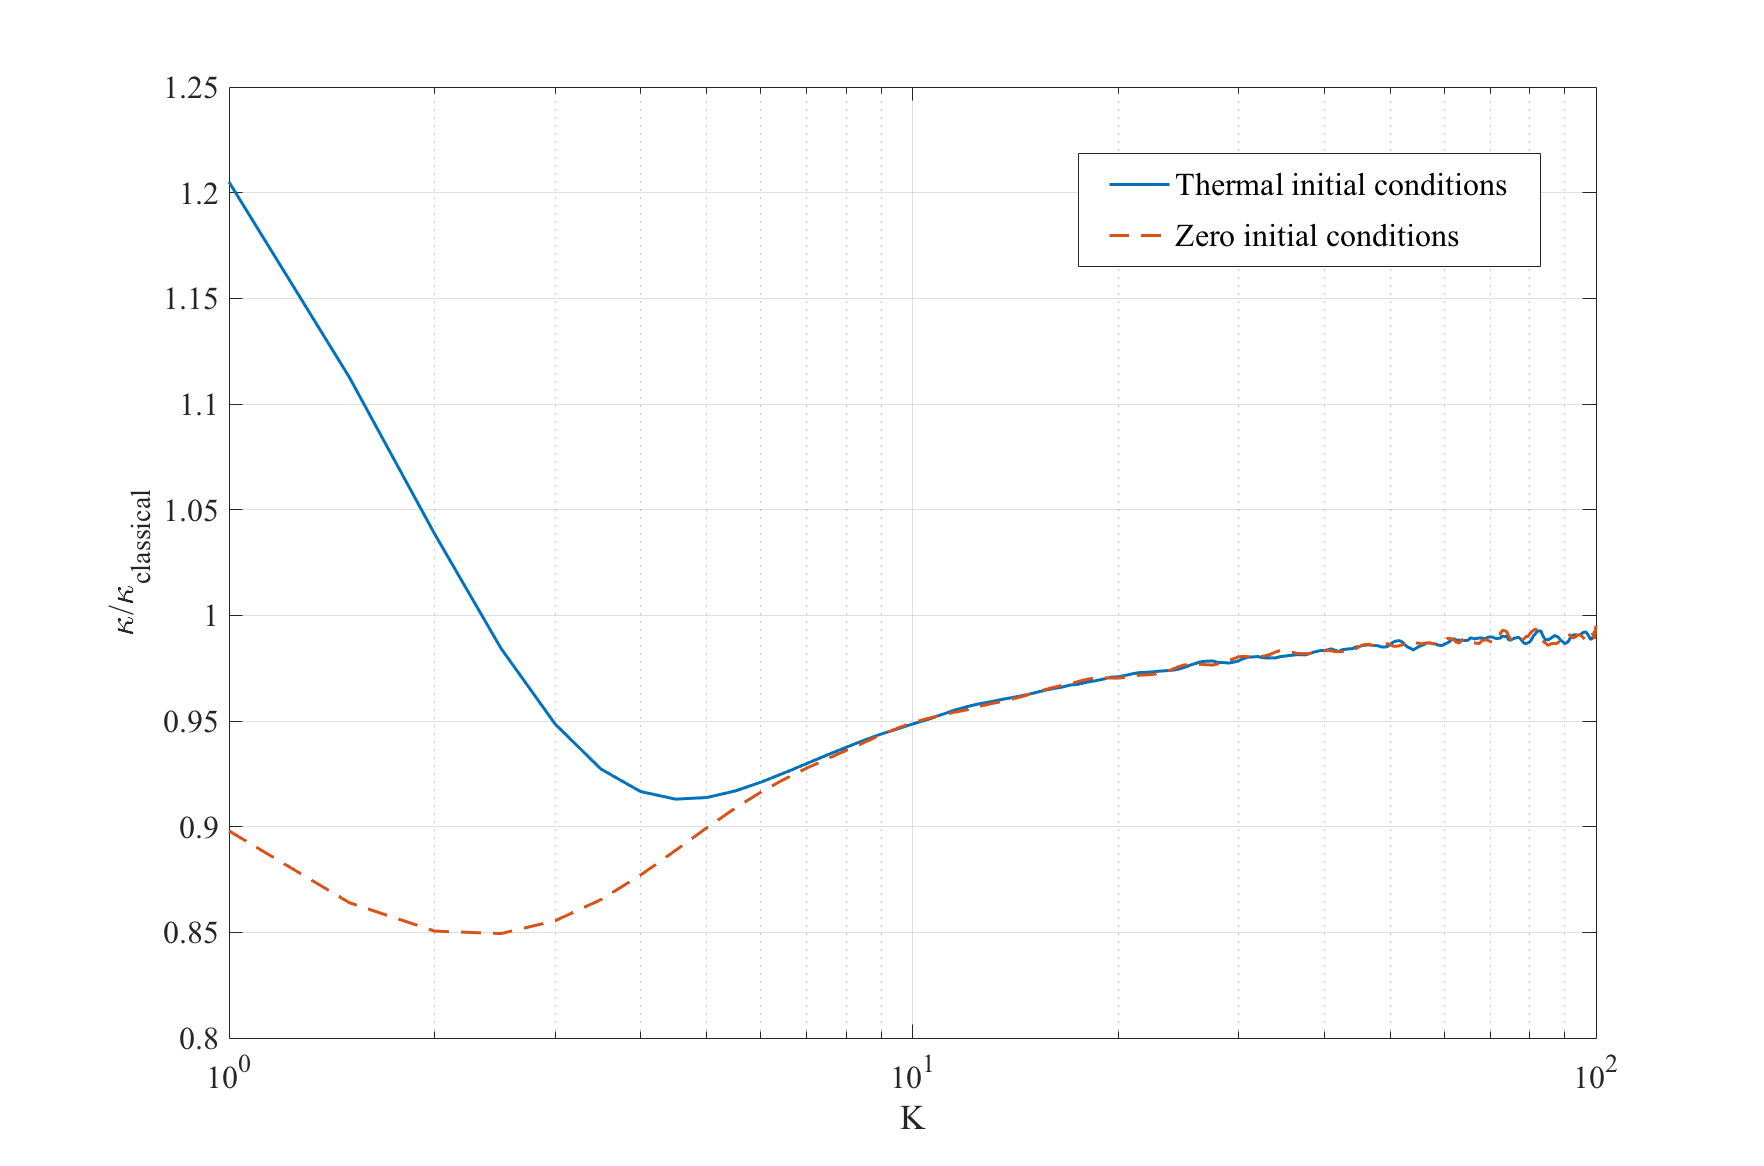
\includegraphics[width=\linewidth]{Images/quantum1}
	\caption{The final efficiency factor determined using only the respective quantum stastics for obtaining $f_\ell f_\phi$ normalized by the final efficiency factor obtained by using classical Boltzmann statistics for thermal and vanishing initial conditions. $c_\ell=1$ and $c_\phi=0$ were used.}
	\label{fig:quantum1}
\end{figure} \noindent
Figure \ref{fig:quantum1} shows how using \eqref{eq:B-L_corrected} instead of \eqref{eq:Gamma_B-l_result} affects the final efficency factor. In general the course of the graphs is similar to the ones in figure \ref{fig:quantum}, however the differences lie in the reached values of the derivation. For $K\sim$1 $\kappa_{classical}$ is about 20\% greater than $\kappa$ for thermal initial conditions and therefore the deviation here is bigger as in \ref{fig:quantum}. For zero initial conditions on the other hand the deviation of about 10\% is comparable to the one above. Now $\kappa_{classical}$ grows bigger with $K$ and surpasses $\kappa$ but the drop of $\kappa/\kappa_{classical}$ is not as severe as above, as it peaks at around 85\% for zero initial conditions and $K\sim$ 2.5, meaning $\kappa_{classical}$ is about 15\% bigger than $\kappa$. For thermal initial conditions this effect is even smaller with the discrepancy between the two efficiency factors, reaching its maximum at around 91\% for $K\simeq$ 5. For both sets of initial conditions this effect gets smaller with growing $K$, so at $K=30$, the point where a nearly constant difference of about 20\% sets in above, the difference is below 2\%. \newline \indent
This is a clear sign showing that in the latter of the cases mentioned above using a classical approximation can have a meaningfull impact on the final efficiency for a low washout parameter, but it slowly gets negligible for higher $K$ in contrast to the first case where the discrepancy between classical and quantum statistics is about 20\% even for high $K$.\newline\indent
Finally, it should be mentioned that the results shown in figure \ref{fig:efficiency}$-$\ref{fig:quantum} agree with the results depicted in Ref. \cite{Bodeker:2013qaa} and \cite{Wormann:2016yyi}.\newpage
	\chapter{Conclusion}
In this thesis the basic principles of electroweak baryogenesis and baryogenesis via leptogenesis, two theoretically possible mechanisms for producing a matter antimatter asymmetry, were presented. It was shown that for both scenarios or for matter antimatter asymmetry creating mechanisms in general the three conditions of baryon number violation, C and CP violation and a departure from the thermal equilibrium, the so called Sakharov coditions, have to be met. \newline \indent
Although the current Standard Model of particle physics could offer everything to meet this conditions in theory, recent experiments have shown that the mass of the Higgs boson is far too heavy to induce a electroweak phase transition of sufficiently strong first order or of first order at all. This phase transition of strong first order, however, is needed to ensure that the non-perturbative B violating processes happen outside of thermal equilibrium. \newline \indent
To circumvent this problem the Standard Model is expanded by heavy, right-handed partners of the nowadays observable light neutrinos. By assuming that neutrinos are Majorana particles, so that they are their own antiparticle, these heavy neutrinos could then decay CP violating into leptons and antileptons, respectively, vioalting lepton number in the process and creating an excess lepton number. For sufficiently high temperatures this lepton number can then be transformed into an excess baryon number by B+L violating processes. This baryon number is then frozen out as soon as the temperature is low enough for the inverse decay to be strongly Boltzmann suppressed. This is known as baryogenesis via leptogenesis. \newline \indent
In addition to this, the rate equations for leptogenesis and the coefficients appearing in these rate equations were obtained in the non-relativistic limit as well as in an expansion including term of up to first order in relativistic corrections. These eqautions were then solved in order to compute the B-L asymmetry in the so called strong washout regime, meaning $K>1$ and the non-relativistic approximation was compared with the relativistic corrections, clearly showing that in the strong washout regime the relative difference between these two is small and that the non-relativistic approximation is a valid one. Also the effect of using different statistics has been computed, showing a far greater influence than the relativistic corrections.  \newline \indent
Finally it can be said that a first hint for verifying the model of leptogenesis would be by experimentally proving the Majorana charakter of neutrinos through processes like the neutrinoless double beta decay. Although no veryified event of such a decay has been observed yet, there is still hope that neutrinos are Majorana particles simply because of the tremendous half-life of $10^{24-25}$ years\cite{Arnold:2016ezh}.

	\appendix
\chapter{The Yukawa interaction term}
\section{Feynman rules for the Yukawa interaction}
In quantum field theories without Majorana particles the Feynman rules for evaluating Feynman diagrams are acquired from the elements of the so called scattering matrix S, given as \cite[Eq. 3.26]{Tong:2006}, given as
\begin{equation}
\lim\limits_{t_\pm\rightarrow\pm\infty}\braket{f|U(t_+,t_-)|i}=\braket{f|S|i}.
\label{eq:s-matrix}
\end{equation}
U(t$_+$,t$_-$) is an unitary time evolution operator explicitly given by Dyson's formula
\begin{equation*}
	U(t_+,t_-)=T\exp\left(-i\int_{t_-}^{t_+}dt\:H_{int}(t)\right).
\end{equation*}
In the following $\psi_{x_i}\equiv\psi(x_i)$ will describe an arbitrary fermionic Dirac, so one can write the time ordering symbol T above in the following way
\begin{equation*}
	T\psi(x)\psi(y)=\left\{\begin{array}{c}\psi(x)\psi(y)\:\:\:\:\:\:\:\:\:\:\text{if } x^0>y^0\\\pm\psi(y)\psi(x)\:\:\:\:\:\:\:\text{if }x^0<y^0\end{array}\right. .
	\end{equation*}
The sign in the lower line depends on if the number of permutations of anticommutating fermion spinors is odd or even. \newline\indent
Using equation \ref{eq:Yukterm} for general fields $\psi$ and $\phi$, the interaction Hamiltonian can be given as
\begin{equation*}
	H_{int}=g\int d^3x \overline{\psi}\psi\phi,
\end{equation*}
with g the coupling constant.\newline\indent
Interesting to note is that, given g is small, by expanding the time evolution operator above one can use quantum mechanical pertubation theory up to an arbitratry order. \newline\indent
Now in order to transform the matrix element into a purely algebraic expression, one first has to reorder the fields $\psi_1$ to $\psi_n$ in a way that the time order symbol T is not needed any more. This can be done using the so called Wick's theorem
\begin{equation*}
	T\left[\psi_1\psi_2\cdots\psi_n\right]=:\psi_1\psi_2\cdots\psi_n+\text{all possible contractions}:.
\end{equation*}
The colon notation simply means that the field operators are normally ordered, meaning all creation operators are on the left side of a product, while the annihilation operators are on the right. The exact mathematical expression of the contraction of two field is not of importance here, but can be looked up for example in section 4.2 of \cite{Kopp:2016}. On the other hand the notation and the final result of such a contraction are vital for the following discussion.
\begin{equation*}
\text{Contraction of $\psi$ and $\overline{\psi}$}=
\contraction{}{\psi}{(x)}{\bar{\psi}}
\psi(x)\overline{\psi}(y)=\braket{0|T[\psi(x)\overline{\psi}(y)]|0}\rightarrow S_F(p).
\end{equation*}
The arrow simply corresponds to the Fourier transformed, since the matrix element above lives in position-space, while it is easier to compute Feynman rules in momentum space. S$_F$(p) is the fermionic Feynman propagator
\begin{equation*}
	S_F(p)=\frac{\left(\slashed p+m\right)}{p^2+m^2+i\epsilon},
\end{equation*}
where the Feynman slash notation
\begin{equation*}
	\slashed p=\gamma^\mu p_\mu
\end{equation*}
was used.
Now, in order to illustrate what the term `all possible contractions' in the Wick theorem above means, this theorem will be applied to a time ordered product of two barred and two unbarred fields will explictily be given
\begin{align*}
		T\left[\psi_1\overline{\psi}_2\psi_3\overline{\psi}_4\right]=\:
		:&\psi_1\overline{\psi}_2\psi_3\overline{\psi}_4+
		\contraction{}{\psi}{{}_1}{\psi}\psi_1\overline{\psi}_2\psi_3\overline{\psi}_4+
		\contraction{}{\psi}{\psi_2{}_3}{\psi}\psi_1\overline{\psi}_2\psi_3\overline{\psi}_4+
		\contraction{}{\psi}{\psi_2\psi_3{}_4}{\psi}\psi_1\overline{\psi}_2\psi_3\overline{\psi}_4+
		\contraction{\psi_1}{\psi}{{}_1}{\psi}\psi_1\overline{\psi}_2\psi_3\overline{\psi}_4+\\
		+\:\contraction{\psi_1}{\psi}{\psi_2{}_3}{\psi}&\psi_1\overline{\psi}_2\psi_3\overline{\psi}_4+
		\contraction{\psi_1\psi_2}{\psi}{{}_4}{\psi}\psi_1\overline{\psi}_2\psi_3\overline{\psi}_4+
		\contraction{}{\psi}{{}_1}{\bar{\psi}}\contraction{\psi_1\psi_2}{\psi}{{}_3}{\bar{\psi}}\psi_1\overline{\psi}_2\psi_3\overline{\psi}_4+
		\contraction{}{\psi}{{}_1\psi_2}{\psi}\contraction[2ex]{\psi_1}{\psi}{{}_2\psi_3}{\psi}\psi_1\overline{\psi}_2\psi_3\overline{\psi}_4+
		\contraction[2ex]{}{\psi}{{}_1\psi_2\psi_3}{\psi}\contraction{\psi_1}{\psi}{{}_2}{\psi}\psi_1\overline{\psi}_2\psi_3\overline{\psi}_4:\:=\\
		=\::&\psi_1\overline{\psi}_2\psi_3\overline{\psi}_4+\contraction{}{\psi}{{}_1}{\psi}\psi_1\overline{\psi}_2\psi_3\overline{\psi}_4+\contraction{}{\psi}{\psi_2\psi_3{}_4}{\psi}\psi_1\overline{\psi}_2\psi_3\overline{\psi}_4+\contraction{\psi_1}{\psi}{{}_1}{\psi}\psi_1\overline{\psi}_2\psi_3\overline{\psi}_4+\contraction{\psi_1\psi_2}{\psi}{{}_4}{\psi}\psi_1\overline{\psi}_2\psi_3\overline{\psi}_4+\\
		+\:\contraction{}{\psi}{{}_1}{\bar{\psi}}\contraction{\psi_1\psi_2}{\psi}{{}_3}{\bar{\psi}}&\psi_1\overline{\psi}_2\psi_3\overline{\psi}_4+\contraction[2ex]{}{\psi}{{}_1\psi_2\psi_3}{\psi}\contraction{\psi_1}{\psi}{{}_2}{\psi}\psi_1\overline{\psi}_2\psi_3\overline{\psi}_4: .
\end{align*}
In the last step the relations
\begin{align}
	\contraction{}{\overline{\psi}}{(x)}{\bar{\psi}}
	\overline{{\psi}}(x)\overline{\psi}(y)=0,
	\label{eq:selfcontraction1}
	\\
	\contraction{}{\psi}{(x)}{\psi}
	\psi(x)\psi(y)=0,
	\label{eq:selfcontraction2}
\end{align}
were used, having the effect that conctracted field are always adjacend to each other in a sense, that to conctraction symbols do not intersect each other. These contractions of just $\psi$ with $\bar{\psi}$ fields can be interpreted as a fermion number flow and therefore the conservation of fermion number. It can be thought of as an incoming particle $\psi$ that becomes an outgoing particle $\bar{\psi}$ after interacting and therefore the fermion number stays the same.\newline\indent
So in order to apply Wicks theorem one has to basically connect two fields pairwise until all possible contractions are performed. \newline\indent
The next important step ist do note that only terms with no uncontracted fields contribute to the corellation function above. In the previous example this means that only the last three terms have to be taken into account in order to obtain the corresponding Feynman rules. \newline\indent
Until now only internal contractions, so contractions of two field operators resulting in the internal propagators, where considered. In order to also take the external, so incoming and outgoing, particles into account one has to take a closer look at the initial and final states $\ket{i}$ and $\bra{f}$. Because in general these states are not just the vacuum, but (multi-)particle states they must consist of creation and anihilation operators acting on the vacuum state, causing contractions of such operators and the fields to arise. Asuming that the particles are not plane waves but rather localized wave packages one can write the states $\ket{i}$ and $\bra{f}$ as\cite{Kopp:2016}
\begin{align*}
\ket{i}=a_1^\dagger a_2^\dagger \cdots b_{n-1}^\dagger b_n^\dagger \ket{0},
\\
\bra{f}=\bra{0}a_1 a_2 \cdots b_{n-1}b_n,
\end{align*}
with the annihilation operators $a_i,b_i$ and the creation operators $a_i^\dagger,b_i^\dagger$ for particles and antiparticles, respectively. The subsript i is short for p$_i$, the particle momentum. In this notations one distinct creation or annihiliation operator can appear twice if two particle with the same momentum are created or destroyed. \newline\indent
Using this and equation \ref{eq:s-matrix}, for a scattering process with a m-particle initial state and a n-particle final state, this results in the following matrix element \cite[Eq. 2.2]{Denner:1992vza}
\begin{equation}
\left<0\left|a_1 a_2 \cdots  b_{n-1} b_n T\left[\left(\bar{\psi}\Gamma\psi\right)\cdots(\bar{\psi}\Gamma\psi\right)]a_{n+1}^\dagger a_{n+2}^\dagger \cdots  b_{m-1}^\dagger b_m^\dagger\right|0\right>.
\label{eq:matrix_element}
\end{equation}
Here the exponential function appearing in the relation above was expanded and only some arbritrary order was chosen, in order to express how the Feynman rules are obtained.\newline\indent
In analogy to the notation in Ref.\cite{Denner:1992vza} $\Gamma$ describes some arbitrary fermionic interaction
\begin{equation*}
	\bar{\psi}\Gamma\psi=g^i_{abc}\bar{\psi}_a\Gamma_i\psi_b\phi_c,
\end{equation*}
with $\Gamma_i=1,i\gamma_5,\gamma_\mu\gamma_5,\gamma_\mu,\sigma_{\mu\nu}$, but for the next discussion $\Gamma_i=1$ will be assumed simply for the sake of clarity. \newline\indent
Applying Wick's Theorem to this new matrix element not only results in the already known propagator terms, but because of the contractions of the fields directly with the creation and annihilation operators one also gets
\begin{align*}
		\bcontraction{}{\psi}{}{a}\psi a_i^\dagger=\braket{0|\psi(x) a_i^\dagger(p,s)|0}&\longrightarrow u(p,s) \text{ incoming particle },\\
		\bcontraction{}{a}{{}_i}{\bar{\psi}}a_i\bar{\psi}=\braket{0|a_i(p,s)\bar{\psi}(x)|0}&\longrightarrow \bar{u}(p,s) \text{ outgoing particle },\\
		\bcontraction{}{\bar{\psi}}{}{b}\bar{\psi} b_i^\dagger=\braket{0|\bar{\psi}(x) b_i^\dagger(p,s)|0}&\longrightarrow \bar{v}(p,s)\text{ incoming antiparticle },\\
		\bcontraction{}{b}{{}_i}{\psi}b_i\bar{\psi}=\braket{0|b_i(p,s)\psi(x)|0}&\longrightarrow v(p,s)\text{ outgoing antiparticle }.
\end{align*}
Here the following expressions for fermion fields
\begin{align*}
\psi=\sum_{s=\pm1/2}\int \frac{d^3p}{2(\pi)^3}\:\frac{1}{2E}\left(a(p,s)u(p,s)e^{-ipx}+b^\dagger(p,s)v(p,s)e^{ipx}\right),\\
\bar{\psi}=\sum_{s=\pm1/2}\int \frac{d^3p}{2(\pi)^3}\:\frac{1}{2E}\left(a^\dagger(p,s)\bar{u}(p,s)e^{ipx}+b(p,s)\bar{v}(p,s)e^{-ipx}\right),
\end{align*}
and the anti-commutator relations
\begin{align*}
		&\{a(p,s),a^\dagger(q,s')\}=\{b(p,s),b^\dagger(q,s')\}=\delta(p-q)\delta_{ss'},\\
		&\{a(p,s),a(q,s')\}=\{b(p,s),b(q,s')\}=0,
\end{align*}
where used to obtain the results above.
In this context $u$, $v$ and their barred versions describe the incoming or outgoing (anti-)particles as seen above, but their exact mathematical expression is of no greater interest here and will therefore not be given. \newline\indent
Shortly summarized the previous discussion shows that, for Dirac particles, using the matrix element \ref{eq:matrix_element} one cannot only determine the internal propagators needed in most processes but also the spinors of incoming and outgoing particles. So a full set of Feynman rules,except for internal,which will not be used, and external scalars,which is trivialy 1, was obtained and can directly be used for calculating the scattering matrix elements for various processes. \newline\indent
However, because the scenario of leptogenesis requires Majorana neutrinos at leas the Feynman rules for exactly this neutrino have to be reiterated. The main difference in obtaining the Feynman rules for Majorana particles in comparison to Dirac particles is that the relations \ref{eq:selfcontraction1} and \ref{eq:selfcontraction2} do no longer hold and therefore contractions of fields not adjacent to each other are possible. It can easy be seen that the same reasoning from above with incoming and outgoing fermions for Dirac particles can not be applied for Majorana particles because of lepton number non-conserving contractions containing just $\psi$ or $\bar{\psi}$ fields.\newline\indent
This problem can be solved by introducing the charge-conjugated particle 
\begin{align*}
	\tilde{\psi}&=C\bar{\psi}^T,\\
	\bar{\tilde{\psi}}&=-\psi^T C^{-1},
\end{align*}
where C is the charge conjugation operator. The interaction term above then becomes the reversed one
\begin{equation*}
		\bar{\psi}\Gamma\psi=g^i_{abc}\bar{\psi}_a\Gamma_i\psi_b\phi_c=(-1)g^i_{abc}\psi_b^T\Gamma_i^T\bar{\psi}_a^T\phi_c=g^i_{abc}\bar{\tilde{\psi}}_aC\Gamma_i^TC^{-1}\tilde{\psi}_b\phi_c=g^i_{abc}\bar{\tilde{\psi}}_a\eta_i\Gamma_i\tilde{\psi}_b\phi_c=:\bar{\tilde{\psi}}\Gamma'\tilde{\psi},
\end{equation*}
with the reversed fermion interaction
\begin{equation*}
	\Gamma'=C\Gamma C^{-1}.
\end{equation*}
In additon the relation
\begin{equation*}
	C\Gamma_i C^{-1}=\eta_i\Gamma_i,
\end{equation*}
with 
\begin{equation*}
	\eta_i=\left\{\begin{array}{c}+1\:\:\:\:\:\:\:\:\:\:\text{for } 1,i\gamma_5,\gamma_\mu\gamma_5\\-1\:\:\:\:\:\:\:\:\:\:\:\:\:\:\:\:\:\text{for }\gamma_\mu,\sigma_{\mu\nu}\end{array}\right.,
\end{equation*}
was used.
Because for Majorana fermions $\tilde{\psi}=\psi$, it is rather easy to notice that the vertex term and the reversed vertex term are the same, $\Gamma'=\Gamma$. \newline\indent
How this untangles intersecting contractions will be shown exemplarily using the following contraction.
\begin{equation*}
	\contraction{}{\bar{\psi}}{{_a\psi_b\:\bar{\psi}_a\psi_b\:\bar{\psi}_a}}{\psi}
	\bcontraction[2ex]{\bar{\psi}_a}{\psi}{{}_b\:\bar{\psi}_a}{\psi}
	\bcontraction{\bar{\psi}_a\psi_b\:}{\bar{\psi}}{{}_a\psi_b\:}{\bar{\psi}}
	\bar{\psi}_a\psi_b\:\bar{\psi}_a\psi_b\:\bar{\psi}_a\psi_b.
\end{equation*}
According to the relation above, we now reverse the middle interaction term and therefore get
\begin{equation*}
	\bar{\psi}_a\psi_b\:\bar{\tilde{\psi}}_b\tilde{\psi}_a\:\bar{\psi}_a\psi_b.
\end{equation*}
Now applying again the contractions, while the same indices as in the original term stay contracted, yields the desired result where all conctracted field are directly next to each other. 
\begin{equation}
\contraction{}{\bar{\psi}}{{_a\psi_b\:\bar{\psi}_a\psi_b\:\bar{\psi}_a}}{\psi}
\bcontraction{\bar{\psi}_a}{\psi}{{}_b\:}{\psi}
\bcontraction{\bar{\psi}_a\psi_b\:\bar{\tilde{\psi}}_b}{\bar{\psi}}{{}_a}{\bar{\psi}}
\bar{\psi}_a\psi_b\:\bar{\tilde{\psi}}_b\tilde{\psi}_a\:\bar{\psi}_a\psi_b.
\label{eq:untangled}
\end{equation}
This can be applied to an arbitrarlily long string of field operators and therefore any combination of general fermion fields can be transformed in a way that is has the same structure as for Dirac fermions, with the only difference being that some fields may be exchanged with their charge conjugated counterparts. As already mentioned, these kind of interaction terms do not conserve fermion number, however, equation \ref{eq:untangled} having the same structure as for Dirac particles the fermion number flow has to be replaced by something else, namely the so called fermiom flow. This fermion flow plays the role of an orientation of a Feynman diagram. This orientation can be chosen arbitrarily, the resulting matrix element are still the same, regardless of the chosen orientation\newline\indent 
The Feynman rules than can be obtained exactly in the same way as for Dirac particles. Using the definition of the charge conjugated fields results in the algebraic expression for the internal propagator given as
\begin{equation*}
	\braket{0|T[\tilde{\psi}\bar{\tilde{\psi}}]|0}=C\braket{0|T[\psi\bar{\psi}]|0}^TC^{-1}\longrightarrow CS(p)^TC^{-1}=\frac{\left(-\slashed p+m\right)}{p^2+m^2+i\epsilon}=S(-p)=:S'(p).
\end{equation*}
Using the explicit expressions for the charge conjugated fields
\begin{align*}
\tilde{\psi}=\sum_{s=\pm1/2}\int \frac{d^3p}{2(\pi)^3}\:\frac{1}{2E}\left(a^\dagger(p,s)u(p,s)e^{-ipx}+b(p,s)v(p,s)e^{ipx}\right)\\
\bar{\tilde{\psi}}=\sum_{s=\pm1/2}\int \frac{d^3p}{2(\pi)^3}\:\frac{1}{2E}\left(a(p,s)\bar{u}(p,s)e^{ipx}+b^\dagger(p,s)\bar{v}(p,s)e^{-ipx}\right)
\end{align*}
 and the exact same anti-commutator relations one gets the analogous results for the external fermion fields;
\begin{align*}
\bcontraction{}{\psi}{}{a}\tilde{\psi} b_i^\dagger=\braket{0|\tilde{\psi}(x) b_i^\dagger(p,s)|0}&\longrightarrow u(p,s); \\
\bcontraction{}{a}{{}_i}{\bar{\psi}}b_i\bar{\tilde{\psi}}=\braket{0|b_i(p,s)\bar{\tilde{\psi}}(x)|0}&\longrightarrow \bar{u}(p,s) ,\\
\bcontraction{}{\bar{\psi}}{}{b}\bar{\tilde{\psi}} a_i^\dagger=\braket{0|\bar{\tilde{\psi}}(x) a_i^\dagger(p,s)|0}&\longrightarrow \bar{v}(p,s),\\
\bcontraction{}{b}{{}_i}{\psi}a_i\bar{\tilde{\psi}}=\braket{0|a_i(p,s)\tilde{\psi}(x)|0}&\longrightarrow v(p,s).
\end{align*}
Summarizing all these results gives a full set of Feynman rules for Majorana as well as Dirac fermions, as they are given in \cite{Denner:1992vza}. For the sake of completeness they will be given here as well. In the following diagramms dotted lines represent a boson field, solid lines without arrows represent Majorana fermions and solid lines with arrows represent Dirac fermions, while the arrow points in the direction of fermion number flow, the thin arrows indicate the fermion flow. The momentum always flows from left to right. 
\begin{figure}[H]
	\begin{subfigure}{\linewidth}
		\begin{equation*}
		\feynmandiagram [small, baseline=(d.base), horizontal=d to b] {
			b -- [edge,thick,momentum'] a,
			b-- [edge,thick,rmomentum] c,
			d   -- [scalar,thick] b}; \quad \sim i\Gamma
		\qquad		
		\feynmandiagram [small, baseline=(d.base), horizontal=d to b] {
			b -- [edge,thick,momentum'] a,
			b-- [anti fermion,thick,rmomentum] c,
			d   -- [scalar,thick] b}; \quad \sim i\Gamma
		\qquad
		\feynmandiagram [small, baseline=(d.base), horizontal=d to b] {
			b -- [fermion,thick,momentum'] a,
			b-- [edge,thick,rmomentum] c,
			d   -- [scalar,thick] b}; \quad \sim i\Gamma
		\qquad
		\feynmandiagram [small, baseline=(d.base), horizontal=d to b] {
			b -- [fermion,thick,momentum'] a,
			b-- [anti fermion,thick,rmomentum] c,
			d   -- [scalar,thick] b}; \quad \sim i\Gamma
		\end{equation*}
	\end{subfigure}
\begin{subfigure}{\linewidth}
	\begin{equation*}
	\feynmandiagram [small, baseline=(d.base), horizontal=d to b] {
		b -- [edge,thick,rmomentum'] a,
		b-- [edge,thick,momentum] c,
		d   -- [scalar,thick] b}; \quad \sim i\Gamma'
	\qquad		
	\feynmandiagram [small, baseline=(d.base), horizontal=d to b] {
		b -- [edge,thick,rmomentum'] a,
		b-- [anti fermion,thick,momentum] c,
		d   -- [scalar,thick] b}; \quad \sim i\Gamma'
	\qquad
	\feynmandiagram [small, baseline=(d.base), horizontal=d to b] {
		b -- [fermion,thick,rmomentum'] a,
		b-- [edge,thick,momentum] c,
		d   -- [scalar,thick] b}; \quad \sim i\Gamma'
	\qquad
	\feynmandiagram [small, baseline=(d.base), horizontal=d to b] {
		b -- [fermion,thick,rmomentum'] a,
		b-- [anti fermion,thick,momentum] c,
		d   -- [scalar,thick] b}; \quad \sim i\Gamma'
	\end{equation*}
\end{subfigure}
	\caption{Feynman rules for fermionic vertices}
	\label{fig:Feynman_veritces}
\end{figure}
\begin{figure}[H]
	\begin{equation*}
	\feynmandiagram [small, baseline=(d.base), horizontal=a to b] {
		a[dot]-- [fermion,thick,momentum'] b[dot] }; \quad \sim iS(p)
	\qquad		
	\feynmandiagram [small, baseline=(d.base), horizontal=a to b] {
		a[dot]-- [fermion,thick,rmomentum'] b[dot] }; \quad \sim iS(-p)
	\qquad		
	\feynmandiagram [small, baseline=(d.base), horizontal=a to b] {
		a[dot] -- [edge,thick,momentum'] b[dot]}; \quad \sim iS(p)
	\end{equation*}
	\caption{Feynman rules for internal fermionic propagators}
	\label{fig:Feynman_intprop}
\end{figure}
\begin{figure}[H]
	\begin{subfigure}{\linewidth}
		\begin{equation*}
		\feynmandiagram [small, baseline=(d.base), horizontal=a to b] {
			a[dot]-- [fermion,thick,momentum'] b};
		\qquad		
		\feynmandiagram [small, baseline=(d.base), horizontal=a to b] {
			a[dot]-- [anti fermion,thick,momentum'] b};
		\qquad		
		\feynmandiagram [small, baseline=(d.base), horizontal=a to b] {
			a[dot] -- [edge,thick,momentum'] b}; 
		\quad
		\sim\bar{u}(p,s)
		\end{equation*}
	\end{subfigure}
	\begin{subfigure}{\linewidth}
		\begin{equation*}
		\feynmandiagram [small, baseline=(d.base), horizontal=a to b] {
			a[dot]-- [fermion,thick,rmomentum'] b};
		\qquad		
		\feynmandiagram [small, baseline=(d.base), horizontal=a to b] {
			a[dot]-- [anti fermion,thick,rmomentum'] b};
		\qquad		
		\feynmandiagram [small, baseline=(d.base), horizontal=a to b] {
			a[dot] -- [edge,thick,rmomentum'] b}; 
		\quad
		\sim v(p,s)
		\end{equation*}
	\end{subfigure}
	\begin{subfigure}{\linewidth}
		\begin{equation*}
		\feynmandiagram [small, baseline=(d.base), horizontal=a to b] {
			a-- [fermion,thick,momentum'] b[dot]};
		\qquad		
		\feynmandiagram [small, baseline=(d.base), horizontal=a to b] {
			a-- [anti fermion,thick,momentum'] b[dot]};
		\qquad		
		\feynmandiagram [small, baseline=(d.base), horizontal=a to b] {
			a -- [edge,thick,momentum'] b[dot]}; 
		\quad
		\sim u(p,s)
		\end{equation*}
	\end{subfigure}
	\begin{subfigure}{\linewidth}
		\begin{equation*}
		\feynmandiagram [small, baseline=(d.base), horizontal=a to b] {
			a-- [fermion,thick,rmomentum'] b[dot]};
		\qquad		
		\feynmandiagram [small, baseline=(d.base), horizontal=a to b] {
			a-- [anti fermion,thick,rmomentum'] b[dot]};
		\qquad		
		\feynmandiagram [small, baseline=(d.base), horizontal=a to b] {
			a -- [edge,thick,rmomentum'] b[dot]}; 
		\quad
		\sim \bar{v}(p,s)
		\end{equation*}
	\end{subfigure}
	\caption{Feynman rules for external fermion lines}
	\label{fig:external_lines}
\end{figure}
\section{The tree level decay rate for heavy neutrinos}
\label{ap:tree_level_decay}
In this section the heavy neutrion decay rate given in equation \ref{eq:Gamma_N} will be calculated using the tree level diagramms in figure \ref{fig:N-decay}, which, for the sake of clarity, will be given here once more, but also with arrows showing the arbitrarily chosen orientation
	\begin{equation*}
	\feynmandiagram [small,baseline=(d.base), horizontal=d to b] {
		b -- [scalar,thick, edge label=\(\overline{\phi}\)] a,
		b-- [fermion,thick, edge label =\(\ell\),momentum'] c,
		d   -- [thick, edge label=N,momentum'] b}; 
	\qquad \text{or} \qquad
	\feynmandiagram [small,baseline=(d.base), horizontal=d to b] {
		b -- [scalar, thick, edge label = \(\phi\)] a,
		b-- [anti fermion, thick,edge label=\(\overline{\ell}\),momentum'] c,
		d  --[thick,edge label=N,momentum'] b  }; 
	\end{equation*}
In general the decay rate can be obtained using
\begin{equation*}
\Gamma=\int d\Gamma,
\end{equation*}
with the differential decay rate given as
\begin{equation*}
d\Gamma=\frac{1}{2M_N}\left|\mathcal{M}\right|^2\frac{d^3p_\ell}{(2\pi)^32E_\ell}\frac{d^3p_\phi}{(2\pi)^32E_\phi}(2\pi)^4\delta^4\left(p_\ell+p_\phi-p_N\right).
\end{equation*}
$\left|\mathcal{M}\right|$ denotes the matrix element corresponding to exactly this decay, that can be read of directly from the corresponding Feynman diagram. 
Now, using the Feynman rules obtained in the previous section one has to first formulate this matrix element in order to be able to evaluate it. Choosing an arbitrary orientation the matrix element for the decay into $\bar{\phi}$ and a lepton reads
\begin{equation*}
i\mathcal{M}=\bar{u}_{\ell_a}(p_{\ell_a},s_{\ell_a})ih_{a1}P_Ru_N(p_N,s_N),
\end{equation*}
where the subscripts $\ell_a$ and N describe the lepton of flavor a and heavy neutrino, respectively and
\begin{equation*}
	P_R=\frac{1+\gamma^5}{2} \qquad P_L=\frac{1-\gamma^5}{2}
\end{equation*}
the chirality operators with $\gamma^5=\gamma^0\gamma^1\gamma^2\gamma^3\gamma^4$, where $\gamma^i$ denotes the gamma matrices. This can be used because the heavy neutrino N, per defnition, is right-handed.
Then the respective absolute square of this matrix element is 
\begin{equation*}
|\mathcal{M}|^2=\bar{u}_{\ell_a}(p_{\ell_a},s_{\ell_a})h_{a1}P_Ru_N(p_N,s_N)\:\bar{u}_{N}(p_{N},s_{N})P_Lih^*_{a1}u_{\ell_a}(p_{\ell_a},s_{\ell_a}).
\end{equation*} \newline\indent
However, this matrix element only describes the decay of a neutrino with a certain spin into a lepton of another certain spin. In order to generalize this for unknown spins of the lepton as well as of the spin one has to sum over the final spins of the lepton and average over the initial spin of the neutrino, resulting in
\begin{equation*}
|\mathcal{M}|^2=2\cdot\frac{1}{2}\sum_{s_N,s_{\ell_a}}\bar{u}_{\ell_a}(p_{\ell_a},s_{\ell_a})h_{a1}P_Ru_N(p_N,s_N)\:\bar{u}_{N}(p_{N},s_{N})P_Lih^*_{a1}u_{\ell_a}(p_{\ell_a},s_{\ell_a}).
\end{equation*}
The factor of 2 arises from the fact that general leptons are part of a weak isospin doublet, so there are two possible values for the isospin, or more precise, its third component, namely T$_3$=-1/2 for the charged leptons e, $\mu$, $\tau$ and T$_3$=1/2 for the corresponding light neutrinos $\nu_{e,\mu,\tau}$. If we just looked at the decay into for example the light neutrinos this factor of 2 has to be omitted since there is only one isospin component T$_3$ possible. Additionally, the heavy neutrino doesn't contribute to this factor because it is a weak isospin singulett and therefore only T$_3$=0 is possible. \newline\indent
In the following we only consider the decay into one lepton flavor a=1, taking more flavors into account simply means summing the following result with different coupling constants h$_{a1}$ for each lepton flavor. This results in
\begin{align*}
|\mathcal{M}|^2&=\sum_{s_N,s_{\ell}}\bar{u}_{\ell}(p_{\ell},s_{\ell})h_{11}P_Ru_N(p_N,s_N)\:\bar{u}_{N}(p_{N},s_{N})P_Lih^*_{11}u_{\ell}(p_{\ell},s_{\ell})=\\
&=|h_{11}|^2\sum_{s_N,s_{\ell}}\bar{u}_{\ell}(p_{\ell},s_{\ell})_\nu\, P_R^{\nu\mu}\,u_N(p_N,s_N)_\mu\:\bar{u}_{N}(p_{N},s_{N})_\alpha\, P_L^{\alpha\beta}\,u_{\ell}(p_{\ell},s_{\ell})_\beta=\\
&=|h_{11}|^2\sum_{s_{\ell}}\bar{u}_{\ell}(p_{\ell},s_{\ell})_\nu\, P_R^{\nu\mu}\,(\slashed p_N+M_N)_{\mu\alpha}\, P_L^{\alpha\beta}\,u_{\ell}(p_{\ell},s_{\ell})_\beta=\\
&=|h_{11}|^2P_R^{\nu\mu}\,(\slashed p_N+M_N)_{\mu\alpha}\, P_L^{\alpha\beta}\,(\slashed p_\ell+M_\ell)_{\beta\nu}=\\
&=|h_{11}|^2\,\text{Tr}\left[P_R\,(\slashed p_N+M_N)\, P_L\,\slashed p_\ell\right],
\end{align*}
with $\nu,\mu,\alpha,\beta$ being spinor indices.\newline\indent
The way this trace was obtained is commonly known as the Casimir trick, which uses the following relation
\begin{equation*}
	\sum_s u(p,s)\bar{u}(p,s)=\slashed p +m,
\end{equation*}
with m being the mass of the particle. \newline\indent
Because the leptons are relativistic their mass can be neglected, what was done in the last step above.\newline\indent
The trace now simplifies to
\begin{align*}
	\text{Tr}\left[P_R\,(\slashed p_N+M_N)\, P_L\,\slashed p_\ell\right]&=\frac{1}{4}\text{Tr}\left[\left(1+\gamma^5\right)\,(\slashed p_N+M_N)\,\left(1-\gamma^5\right)\,\slashed p_\ell\right]=\\
	&=\frac{1}{4}\left(\text{Tr}\left[\gamma^\mu (p_N)_\mu \gamma^\nu (p_\ell)_\nu\right]+ \text{Tr}\left[M\gamma^\mu (p_\ell)_\mu\right]+\right.\\ 
	&+\text{Tr}\left[\gamma^5\gamma^\mu (p_N)_\mu\gamma^\nu (p_\ell)_\nu\right]+ \text{Tr}\left[M\gamma^5\gamma^\mu (p_\ell)_\mu\right]-\\
	 &-\text{Tr}\left[\gamma^\mu (p_N)_\mu\gamma^5\gamma^\nu (p_\ell)_\nu\right]- \text{Tr}\left[M\gamma^5\gamma^\mu (p_\ell)_\mu\right]-\\
	  &\left.-\text{Tr}\left[\gamma^5\gamma^\mu (p_N)_\mu\gamma^5\gamma^\nu (p_\ell)_\nu\right]- \text{Tr}\left[M\gamma^5\gamma^5\gamma^\mu (p_\ell)_\mu\right] \right)=\\
	&=\frac{1}{4}\text{Tr}\left[\gamma^\mu (p_N)_\mu\gamma^\nu (p_\ell)_\nu\right]-\frac{1}{4}\text{Tr}\left[\gamma^5\gamma^\mu (p_N)_\mu\gamma^5\gamma^\nu (p_\ell)_\nu\right]=\\
	&=\frac{1}{2}\text{Tr}\left[\gamma^\mu (p_N)_\mu\gamma^\nu (p_\ell)_\nu\right]=\frac{1}{2}\text{Tr}\left[\slashed p_N \slashed p_\ell\right].
\end{align*}
All of the terms, aside from the first and second to last one, vanished because of the following relations:
\begin{equation*}
	\text{Tr}\left[\gamma^\mu\right]=0; \qquad \text{Tr}\left[\gamma^\mu\gamma^\nu\gamma^5\right]=0;\qquad \text{Tr}\left[\text{odd number of $\gamma$'s}\right]=0
\end{equation*}
The final relation necessary to finally evaluate the trace is
\begin{equation*}
	\text{Tr}[\gamma^\mu\gamma^\nu]=4\eta^{\mu\nu},
\end{equation*}
as well as the Minkowski metric $\eta^{\mu\nu}$. Using this one gets the final result for the squared matrix element
\begin{equation*}
	|\mathcal{M}|^2=\frac{1}{2}|h_{11}|^2\text{Tr}\left[\slashed p_N \slashed p_\ell\right]=2|h_{11}|^2(p_N)_\mu (p_\ell)_\nu\eta^{\mu\nu}=2|h_{11}|^2p_Np_\ell.
\end{equation*}
In order to rewrite the product of the 4-momentum vectors the decay will be treated in the center of mass system, meaning $p_N=(M_N,\vec{0})$. Additionally, treating the leptons as relativistic particles, so $p_\ell=(|\vec{p}_\ell|,\vec{p}_\ell)$, results in
\begin{equation*}
|\mathcal{M}|^2=2|h_{11}|^2p_Np_\ell=2|h_{11}|^2M_N|\vec{p}_\ell|.
\end{equation*}
But due to the neutrino not only decaying into leptons but also into anti-leptons this is not the whole contribution to the tree level decay rate. However, looking at figure \ref{fig:external_lines}, the corresponding matrix element looks exactly the the same and therefore would contribute the same term to the decay rate. This result is not surprising, remembering that CP violation only arises through interference of tree level and one-loop diagrams, thus $\Gamma(N\rightarrow\bar{\phi}\ell)=\Gamma(N\rightarrow\phi\bar{\ell})$. Plugging both these contribution back into the relation for the total decay rate results in 
\begin{align*}
	\Gamma&=\frac{1}{2M_N}\int\frac{d^3p_\ell}{(2\pi)^32E_\ell}\frac{d^3p_\phi}{(2\pi)^32E_\phi}(2\pi)^44|h_{11}|^2M_N|\vec{p}_\ell|\delta^4\left(p_\ell+p_\phi-p_N\right)=\\
	&=\frac{1}{8\pi^2}\int\frac{d^3p_\ell}{E_\ell}\frac{d^3p_\phi}{E_\phi}|h_{11}|^2M_N|\vec{p}_\ell|\delta\left(|\vec{p}_\ell|+|\vec{p}_\phi|-M_N\right)\delta^3\left(\vec{p}_\ell+\vec{p}_\phi\right)=\\
	&=\frac{|h_{11}|^2}{8\pi^2}\int\frac{d^3p_\ell}{E_\ell}\frac{1}{E_\phi}|\vec{p}_\ell|\delta\left(2|\vec{p}_\ell|-M_N\right)=\\
	&=\frac{|h_{11}|^2}{8\pi^2}\int\frac{d^3p_\ell}{p_\ell}\delta\left(2|\vec{p}_\ell|-M_N\right).
\end{align*}
To get to the third line the 3-momentum delta function was used, resulting in $\vec{p}_N=-\vec{p}_\ell$. Also, since the Higgs particles and leptons are relativistic their energies can be replaced by the absolute value of their momentum. To solve the last remaining integral, one has to use the final delta function.
\begin{align*}
	\Gamma&=\frac{|h_{11}|^2}{8\pi^2}\int\frac{d^3p_\ell}{p_\ell}\delta\left(2|\vec{p}_\ell|-M_N\right)=\\
	&=\frac{|h_{11}|^2}{2\pi}\int_0^{\infty} dp_\ell \:p_\ell\delta\left(2|\vec{p}_\ell|-M_N\right)=\\
	&=\frac{|h_{11}|^2}{2\pi}\int_0^{\infty} \frac{dx}{4}\:x\delta\left(x-M_N\right)=\\
	&=\frac{|h_{11}|^2}{8\pi}M_N.
\end{align*}
\chapter{Detailed calculations}
\section{Integrating the rate equation over phase space}
\label{ap:phase_space}
In order to be able to determine $\Gamma_N$ it is usefull to perform the phase space integral over following equation:
\begin{equation*}
\left(\frac{d}{dt}+3H\right)n_N=-\Gamma_N\left(n_N-n_N^{eq}\right).
\end{equation*}
Comparing this to \ref{eq:L_rate_expanding_interaction} one sees that the second term on the right-hand side has already been omitted since it is, as stated above, small enough to be safely neglected. \newline\indent
Now perfomring the phase space integral results in
\begin{align*}
\int\frac{d^3p}{\left(2\pi\right)^3}\: \left(\frac{d}{dt}+3H\right)f_N=-\int\frac{d^3p}{\left(2\pi\right)^3}\:\Gamma_N\left(f_N-f_N^{eq}\right)\\
\Rightarrow \int dp\: \left(\frac{d}{dt}+3H\right)f_Np^2=-\int dp\:\Gamma_N\left(f_N-f_N^{eq}\right)p^2.
\end{align*}
Using the following partial integration to evaluate the left-hand side
\begin{equation*}
\int dp\:p^3\frac{\partial f_N}{\partial p}=\left[p^3f_N\right]_0^\infty-3\int dp\:p^2f_Ndp=-3\int p^2f_N,
\end{equation*}
\begin{equation*}
3H\int dp\: f_Np^2=-H\int dp\: p^3\frac{\partial f_N}{\partial p},
\end{equation*}
it follows that
\begin{align*}
\int  dp\:\left(\partial_t-Hp\partial_p\right)f_Np^2&=-\int dp\:\Gamma_N\left(f_N-f_N^{eq}\right)p^2\\
\Rightarrow \left(\partial_t-Hp\partial_p\right)f_N&=\Gamma_N\left(f_N^{eq}-f_N\right).
\end{align*}
\section{Detailed calculation of $\Gamma_{B-L}$}
\label{ap:Gamma_B-L}
First the rather simple derivation of \ref{eq:distri_diff} shall be displayed here. For the product of two Boltzman factors one has
\begin{equation*}
f_\ell^{eq}f_\phi^{eq}=e^{-\frac{E_\ell-\mu_\ell}{T}}e^{-\frac{E_\phi-\mu_\phi}{T}}=e^{-\frac{E_N-\mu_\ell-\mu_\phi}{T}}=e^{-\frac{E_N}{T}}e^{\frac{\mu_\ell+\mu_\phi}{T}},
\end{equation*}
where the relation E\textsubscript{$\ell$}+E\textsubscript{$\phi$}=E\textsubscript{N} was used. \newline\indent
Expanding this up to first order in the chemical potential results in
\begin{equation*}
f_\ell f_\phi\simeq e^{-\frac{E_N}{T}}\left(1+\frac{\mu_\ell+\mu_\phi}{T}\right).
\end{equation*}
Finally putting this togehter for leptons and Higgs particles and using the relation $\mu_X=-\mu_{\bar{X}}$ for the chemical potentials of a particle X and its anti particle X yields the result presented above,
\begin{equation*}
f_lf_\phi-f_{\bar{l}}f_{\bar{\phi}}\simeq e^{-\frac{E_N}{T}}\left(1+\frac{\mu_l+\mu_\phi}{T}-1-\frac{\mu_{\bar{l}}+\mu_{\bar{\phi}}}{T}\right)=2e^{-\frac{E_N}{T}}\frac{\mu_l+\mu_\phi}{T}.
\end{equation*}
\newline\indent
Now, as already explained, in order to relate the chemicial potentials to the density n\textsubscript{B-L} one has to expand the left-hand side of \ref{eq:l-lbar} and \ref{eq:phi-phibar} up to first order in the chemical potentials while using Fermi-Dirac and Bose-Einstein distributions instead of Boltzmann statistics, yielding
\begin{align*}
	n_\ell-n_{\bar{\ell}}&=g_\ell\int\frac{d^3p}{\left(2\pi\right)^3}f_\ell-f_{\bar{\ell}}=\\
	&=g_\ell\frac{1}{\left(2\pi\right)^3}\int dp\:dcos\theta \:d\phi\left(f_\ell-f_{\bar{\ell}}\right)p^2=\\
	&=g_\ell\frac{1}{2\pi^2}\int dp \: \left(f_\ell\left(\mu_\ell=0\right)+\frac{e^{E/T}}{\left(e^{E/T}+1\right)^2T}\mu_\ell-f_{\bar{\ell}}\left(\mu_{\bar{l}}=0\right)-\frac{e^{E/T}}{\left(e^{E/T}+1\right)^2T}\mu_{\bar{\ell}}\right)p^2=\\
	&=g_\ell\frac{1}{2\pi^2}\int dp\: \frac{2e^{E/T}}{\left(e^{E/T}+1\right)^2T}\mu_\ell p^2=\\
	&=g_\ell\frac{\mu_\ell}{\pi^2T}\int_{0}^{\infty}dE\:\frac{2e^{E/T}}{\left(e^{E/T}+1\right)^2}\:E^2=\\
	&=\frac{\mu_\ell T^2}{3}.
\end{align*}
Analogous calculation for the Higgs yields:
\begin{align*}
	n_\phi-n_{\bar{\phi}}=\frac{2\mu_\phi T^2}{3}.
\end{align*}
Here the degrees of freedom g$_\ell=2=$ g$_\phi$ were used for leptons as well as for the Higgs. \newline\indent
Solving \ref{eq:l-lbar} and \ref{eq:phi-phibar} for the chemical potentials results in
\begin{align*}
	\mu_\ell=\frac{3c_\ell}{T^2}n_{B-L},\\
	\mu_\phi=\frac{3c_\phi}{2T^2}n_{B-L}.
\end{align*}
Plugging all these results into \ref{eq:Gamma_B-L} one gets the following relation
\begin{align*}
	\Gamma_{B-L}&=\frac{3}{8\pi^4}\:\left(c_\ell+\frac{c_\phi}{2}\right)\:\frac{M_N}{T^3}\Gamma_0\int\prod_{a=N,\ell,\phi}\frac{d^3p_a}{E_a}\delta^4\left(p_\ell+p_\phi-p_N\right)e^{-\frac{E_N}{T}}=\\
	&=\frac{3}{8\pi^4}\:\left(c_\ell+\frac{c_\phi}{2}\right)\:\frac{M_N}{T^3}\Gamma_0\int \frac{d^3p_N}{E_N}e^{-\frac{E_N}{T}}\left(\int\frac{d^3p_\ell}{E_\ell}\frac{d^3p_\phi}{E_\phi}\delta^4\left(p_\ell+p_\phi-p_N\right)\right).
\end{align*}
For the sake of minimizing the writing of redundant coefficients we first will evaluate the two body decay phase space in the parentheses above. For simplification the frame of reference used will be the rest frame of the neutrino $\vec{p}_N=0$.
\begin{align*}
\int\frac{d^3p_\ell}{E_\ell}\frac{d^3p_\phi}{E_\phi}\delta^4\left(p_\ell+p_\phi-p_N\right)&=\int\frac{d^3p_\ell}{E_\ell}\frac{d^3p_\phi}{E_\phi}\delta\left(E_\ell+E_\phi-M_N\right)\delta^3\left(\vec{p}_\ell+\vec{p}_\phi\right)=\\
&=\int\frac{d^3p}{E_\ell}\frac{1}{E_\phi}\delta\left(E_\ell+E_\phi-M_N\right)
\end{align*}
From the first to the second line using the delta distribution for the particle momenta yields $\vec{p}\equiv\vec{p}_\ell=-\vec{p}_\phi$. Also by introducing E $\equiv E_\ell+E_\phi$ and using spherical coordinates and the following change of integration variables
\begin{align*}
	E=E_\ell+E_\phi=\sqrt{M_\ell+p^2}+\sqrt{M_\phi+p^2} \Longrightarrow \frac{dE}{dp}=\frac{p}{E_\ell}+\frac{p}{E_\phi} \\
	\Longrightarrow dp=\left(\frac{p}{E_l}+\frac{p}{E_\phi}\right)^{-1}dE=\frac{E_\ell E_\phi}{pE_\ell+pE_\phi}dE=\frac{E_\ell E_\phi}{pE}dE,
\end{align*}
one gets
\begin{align*}
	4\pi\int dE\: \frac{p^2}{pE}\delta\left(E-M_N\right)=4\pi\int dE\: \frac{p}{E}\delta\left(E-M_N\right)=4\pi\frac{p}{M_N}=2\pi \frac{M_N}{M_N}=2\pi
\end{align*}
In order to evaluate the last integral one has to use the delta distribution, resulting in E=M\textsubscript{N}, while the last step uses the fact that leptons and Higgs are relativistic and therefore their energy is E$_{\ell,\phi}\approx$ p and in addition that the energy needed for the inverse decay to be possible in the neutrino's rest frame has to be E$_{\ell,\phi}\approx p=\frac{M\textsubscript{N}}{2}$. Finally plugging this into the original relation for $\Gamma_{B-L}$ yields
\begin{align*}
	\Gamma_{B-L}&=\frac{3}{8\pi^4}\:\left(c_\ell+\frac{c_\phi}{2}\right)\:\frac{M_N}{T^3}\Gamma_0\int \frac{d^3p_N}{E_N}e^{-\frac{E_N}{T}} \cdot 2\pi=\\
	&=\frac{3}{\pi^2}\:\left(c_\ell+\frac{c_\phi}{2}\right)\:\frac{M_N}{T^3}\Gamma_0\int_0^\infty \frac{dp_N}{E_N}\:p_N^2e^{-\frac{E_N}{T}}.
\end{align*}
And with the final change of integration variables 
\begin{align*}
	x=\sqrt{\frac{p_N^2}{M_N^2}+1}\Longrightarrow p_N=\sqrt{x^2-1}M_N \Longrightarrow dp_N=\frac{x}{\sqrt{x^2-1}}M_Ndx,
\end{align*}
one gets 
\begin{align*}
	\Gamma_{B-L}&=\frac{3}{\pi^2}\:\left(c_\ell+\frac{c_\phi}{2}\right)\:\frac{1}{T^3}\Gamma_0\int_{1}^{\infty}dx\: \frac{\left(x^2-1 \right)M_N^2}{M_N\cdot x}\cdot \frac{x}{\sqrt{x^2-1}}\cdot M_N e^{-zx}=\\
	&=\frac{3}{\pi^2}\:\left(c_\ell+\frac{c_\phi}{2}\right)z^3\Gamma_0\int_{1}^{\infty}dx\: \sqrt{x^2-1}e^{-zx}=\\
	&=\frac{3}{\pi^2}\:\left(c_\ell+\frac{c_\phi}{2}\right)z^2K_1(z)\Gamma_0,
\end{align*}
where in the last step the definition of the modified Bessel function of the second kind was used:
\begin{equation*}
	K_n(z)=\frac{\sqrt{\pi}}{\Gamma\left(n+\frac{1}{2}\right)}\left(\frac{1}{2}z\right)^n\int_{1}^{\infty}dx\:\left(x^2-1\right)^{n-\frac{1}{2}}e^{-zx}.
\end{equation*}
With $\Gamma(n)$ the gamma function as generalization of the factorial.
\section{Obtaining relativistic corrections to the rate equations}
\label{ap:rel_corrections}
Expanding the factor 1/E$_N$ on the right-hand side of \ref{eq:L_rate_expanding_interaction_rel} by using \ref{eq:rel_energy_momentum} up to order p$^2$, one gets
\begin{align*}
		\left(\frac{\partial}{\partial t}-Hp\frac{\partial}{\partial p}\right)f_N=\Gamma_0\left(f_N^{eq}-f_N\right)-\frac{\Gamma_0}{2}\left(\frac{p_N}{M_N}\right)^2\left(f_N^{eq}-f_N\right).
\end{align*}
Now integrating over p and using the definition of u given in \ref{eq:energy_density} the right-hand side simplifies to
\begin{equation*}
	g_N\int \frac{d^3p}{(2\pi)^3}\left(\Gamma_0\left(f_N^{eq}-f_N\right)-\frac{\Gamma_0}{2}\left(\frac{p_N}{M_N}\right)^2\left(f_N^{eq}-f_N\right)\right)=\Gamma_N\left(n_N^{eq}-n_N\right)+\Gamma_{N,u}\left(u-u^{eq}\right)
\end{equation*}
and it can easily be seen that $\Gamma_{N,u}=\Gamma_{0}$ \newline\indent
The left-hand side however can be evaluated by performing the steps done in \ref{ap:phase_space}, but in reverse order. \newline\indent
The next thing to do is acquiring the rate equation for u and therefore one has to multiply equation \ref{eq:L_rate_expanding_interaction_rel} with p$^2$ and integrate over p. At leading order $\left(E_N=M_N\left[1+\mathcal{O}(p^2)\right]\right)$ in p this yields
\begin{align*}
	g_N\int \frac{d^3p}{(2\pi)^3\:M_N}\:\left(p^2\frac{\partial}{\partial t}-Hp^3\frac{\partial}{\partial p}\right)f_N=\Gamma_0\:g_N\int \frac{d^3p}{M_N}\left(e^{E_N/T}-f_N\right)p^2.
\end{align*}
Using the following partial integration
\begin{align*}
	-\int d^3p\:Hp^3\frac{\partial}{\partial p}f_N&=-4\pi\int dp\:Hp^5\frac{\partial}{\partial p}f_N=\\
	&=-4\pi\left(\left[p^5f_N\right]_0^\infty-5\int dp\: p^4f_N\right)=\\
	&=4\pi\int dp\: 5p^4f_N=5\int d^3p\: p^2f_N
\end{align*}
and again the definition of u one easily gets
\begin{equation*}
	\left(\frac{d}{dt}+5H\right)u=\Gamma_u\left(u^{eq}-u\right).
\end{equation*}
with $\Gamma_u=\Gamma_0$ at leading order in p. \newline\indent
By performing the same steps as shown in \ref{ap:phase_space} but applied on equation \ref{eq:B-L_rate_expanding_interaction} one gets an equation equivalent to \ref{eq:boltzmann}. The last part will be neglected in the following since it doesn't matter considering relativistic corrections.
\begin{equation*}
\left(\frac{\partial}{\partial t}-Hp\frac{\partial}{\partial p}\right)f_{B-L}=\frac{M_N\Gamma_{B-L}}{E_N}\left(f_N-e^{-E_N/T}\right)
\end{equation*}
Here the Lorentz invariant phase space was already taken into account.\newline\indent
Analogous to the procedure above one has to only consider the right-hand side of this equation and expanding the factor 1/E$_N$ results in
\todo{Minus klären}
\begin{equation*}
g_N\int \frac{d^3p}{(2\pi)^3}\left(\Gamma_{B-L}\left(f_N-f_N^{eq}\right)-\frac{\Gamma_{B-L}}{2}\left(\frac{p_N}{M_N}\right)^2\left(f_N-f_N^{eq}\right)\right)=\Gamma_{B-L}\left(n_N-n_N^{eq}\right)-\Gamma_{B-L,u}\left(u-u^{eq}\right).
\end{equation*}
Also easy to see is the following relation:
\begin{equation*}
	\Gamma_{B-L,u}=\epsilon\Gamma_0
\end{equation*}
\section{Obtaining radiative corrections to the rate equations}
\label{ap:rad_corrections}
Starting from equation \ref{eq:L_rate_expanding_interaction_rel} one first expresses the number densities through the corresponding distributions and gets
\begin{equation*}
	\left(\frac{\partial}{\partial t}+3H\right)\int\frac{d^3p}{\left(2\pi\right)^3}\:f_N=\Gamma_N\int\frac{d^3p}{\left(2\pi\right)^3}\left(f_N^{eq}-f_N\right)+\frac{\Gamma_{N,u}}{M_N}\int\frac{d^3p}{\left(2\pi\right)^3}\frac{p^2}{2M_N}\left(f_N-f_N^{eq}\right).
\end{equation*}
Since the integration variables and range of integration are the same on both sides the integrals and phase space normalization factors can be dropped. Now assuming that these equations hold for f$_N\rightarrow0$ and using \ref{eq:df_dt} this simplifies to 
\begin{align*}
	f_N^{eq}\Gamma_0\frac{M_N}{E_N}\left(a+\frac{p^2}{M_N^2}b+\mathcal{O}\left(\frac{p^4}{M_N^4}\right)\right)=\Gamma_Nf_N^{eq}-\Gamma_{N,u}\frac{p^2}{M_N^2}f_N^{eq}\\
	\Rightarrow\Gamma_0\frac{M_N}{E_N}\left(a+\frac{p^2}{M_N^2}b+\mathcal{O}\left(\frac{p^4}{M_N^4}\right)\right)=\Gamma_N-\Gamma_{N,u}\frac{p^2}{M_N^2}.
\end{align*}
Now again, expanding the 1/E$_N$ factor yields
\begin{align*}
	\Gamma_0\left(1-\frac{p^2}{M_N^2}\right)\left(a+\frac{p^2}{M_N^2}b+\mathcal{O}\left(\frac{p^4}{M_N^4}\right)\right)=\Gamma_N-\Gamma_{N,u}\frac{p^2}{M_N^2}\\
	\Rightarrow a\Gamma_0-\frac{1}{2}(a-2b)\Gamma_0\frac{p^2}{M_N^2}+\mathcal{O}\left(\frac{p^4}{M_N^4}\right)=\Gamma_N-\Gamma_{N,u}\frac{p^2}{M_N^2}.
\end{align*}
Since equation \ref{eq:L_rate_expanding_interaction_rel} is a relation of order p$^2$ terms of higher order do not need to be taken into account. \newline\indent
Now simply comparing coefficients of the terms of different order in p yields the already known result
\todo{Faktor 2 klären}
\begin{align*}
\Gamma_N=&\Gamma_u=a\Gamma_0,\\
\Gamma_{N,u}=&\frac{1}{2}(a-2b)\Gamma_0.
\end{align*}
Using the same procedure on equation \ref{eq:rate_u} results in 
\begin{align*}
&\left(\frac{\partial}{\partial t}+5H\right)\int\frac{d^3p}{\left(2\pi\right)^3}\frac{p^2}{2M_N^2}\:f_N=\frac{\Gamma_{u}}{M_N}\int\frac{d^3p}{\left(2\pi\right)^3}\frac{p^2}{2M_N}\left(f_N-f_N^{eq}\right)\\
&\overset{f_N\rightarrow0}{\Longrightarrow}f_N^{eq}\Gamma_0\frac{M_N}{E_N}\left(a+\mathcal{O}\left(\frac{p^2}{M_N^2}\right)\right)=\Gamma_{u}\frac{p^2}{M_N^2}f_N^{eq}\\
&\overset{E_N=M_N+\mathcal{O}(p^2)}{\Longrightarrow}\Gamma_u=a\Gamma_0.
\end{align*}
Because equation \ref{eq:rate_u} is only of order p, one can drop all terms of order p$^2$ or higher to obtain this result
\section{Differences between quantum and classical statistics}
\label{ap:statistics}
As mentioned in section \ref{sec:num_results} there are two oppurtunities to chose classical statistics over quantum statistics and vice versa. The first one covered here will be considering equations \eqref{eq:chempot_l} and \eqref{eq:chempot_phi}. In section \ref{ap:Gamma_B-L} quantum statistics were used for that particular matter, so here classical statistics will be used. So by expanding up to first order in chemical potentials one gets 
\begin{align*}
n_\ell-n_{\bar{\ell}}&=g_\ell\int\frac{d^3p}{\left(2\pi\right)^3}f_\ell-f_{\bar{\ell}}=\\
&=g_\ell\frac{1}{\left(2\pi\right)^3}\int dp\:dcos\theta \:d\phi\left(f_\ell-f_{\bar{\ell}}\right)p^2=\\
&=g_\ell\frac{1}{2\pi^2}\int dp \: \left(f_\ell\left(\mu_\ell=0\right)+\frac{e^{E/T}}{T}\mu_\ell-f_{\bar{\ell}}\left(\mu_{\bar{l}}=0\right)-\frac{e^{E/T}}{T}\mu_{\bar{\ell}}\right)p^2=\\
&=g_\ell\frac{1}{2\pi^2}\int dp\: \frac{2e^{E/T}}{T}p^2\mu_\ell=\\
&=g_\ell\frac{\mu_\ell}{\pi^2T}\int_{0}^{\infty}dE\:2e^{E/T}\:E^2=\\
&=-\frac{4\mu_\ell T^2}{\pi^2},
\end{align*}
where $g_ell$=2 was used.
Since Boltzmann statistics do not distinguish between fermions and bosons $n_\phi-n_{\bar{\phi}}=n_\phi-n_{\bar{\phi}}$, yielding
\begin{align*}
\mu_\ell=\frac{\pi^2c_\ell}{4T^2}n_{B-L},\\
\mu_\phi=\frac{\pi^2c_\phi}{4T^2}n_{B-L}.
\end{align*}
Plugging this back into \eqref{eq:Gamma_B-L} and following the same calculation as in \ref{ap:Gamma_B-L} then results in
\begin{align*}
\Gamma_{B-L}&=\frac{1}{32\pi^2}\:\left(c_\ell+\frac{c_\phi}{2}\right)\:\frac{M_N}{T^3}\Gamma_0\int\prod_{a=N,\ell,\phi}\frac{d^3p_a}{E_a}\delta^4\left(p_\ell+p_\phi-p_N\right)e^{-\frac{E_N}{T}}=\\
&=\frac{1}{4}\:\left(c_\ell+\frac{c_\phi}{2}\right)z^2K_1(z)\Gamma_0.
\end{align*}
On the other hand classical Boltzmann statistics were used to attain the factor $f_\ell f_\phi-f_{\bar{\ell}}f_{\bar{\phi}}$. How this factor will be corrected using the respective quantum statistics will be shown now. \newline\indent
The product of these two distribution simply yields
\begin{equation*}
	f_\ell f_\phi=\frac{1}{\left(e^{\left(E_\ell-\mu_\ell\right)/T}+1\right)\left(e^{\left(E_\phi-\mu_\phi\right)/T}-1\right)}.
\end{equation*}
Now using the following derivatives
\begin{align*}
	\frac{\partial}{\partial\mu_\ell}f_\ell f_\phi=\frac{1}{\left(e^{\left(E_\ell-\mu_\ell\right)/T}+1\right)^2\left(e^{\left(E_\phi-\mu_\phi\right)/T}-1\right)}\:\frac{e^{\left(E_\ell-\mu_\ell\right)/T}}{T},\\
	\frac{\partial}{\partial\mu_\phi}f_\ell f_\phi=\frac{1}{\left(e^{\left(E_\ell-\mu_\ell\right)/T}+1\right)\left(e^{\left(E_\phi-\mu_\phi\right)/T}-1\right)^2}\:\frac{e^{\left(E_\phi-\mu_\phi\right)/T}}{T},
\end{align*}
this product can be expanded for small chemical potentials up to linear order.
\begin{equation*}
	f_\ell f_\phi=\frac{1}{\left(e^{E_\ell/T}+1\right)\left(e^{E_\phi/T}-1\right)}\left(1+\frac{e^{E_\phi/T}}{T\left(e^{E_\phi/T}-1\right)}\mu_\phi+\frac{e^{E_\ell/T}}{T\left(e^{E_\ell/T}-1\right)}\mu_\ell\right)+\mathcal{O}(\mu^2)
\end{equation*}
Using this and the relations for the chemical potentials form chapter \ref{ap:Gamma_B-L} one gets
\begin{equation*}
	f_\ell f_\phi-f_{\bar{\ell}} f_{\bar{\phi}}=\frac{6n_{B-L}}{T^3\left(e^{E_\ell/T}+1\right)\left(e^{E_\phi/T}-1\right)}\left(\frac{e^{E_\phi/T}}{e^{E_\phi/T}-1}\:\frac{c_\phi}{2}+\frac{e^{E_\ell/T}}{e^{E_\ell/T}-1}c_\ell\right).
\end{equation*}
where again the relation $\mu_x=\mu_{\bar{x}}$ was used. \newline\indent
It is also easy to see that by neglecting the $\pm$1 terms in the denominators, so for high Higgs and lepton energies, exactly the result that is obtained by using Maxwell-Boltzmann statistics is reproduced. \newline\indent
Putting this back into \ref{eq:Gamma_B-L} results in
\begin{align*}
	\Gamma_{B-L,q}&=\frac{3}{8\pi^4}\:\frac{M_N}{T^3}\Gamma_0\int \frac{d^3p_N}{E_N}\times\\
	&\times\left(\int\frac{d^3p_\ell}{E_\ell}\frac{d^3p_\phi}{E_\phi}\frac{1}{\left(e^{E_\ell/T}+1\right)\left(e^{E_\phi/T}-1\right)}\left(\frac{e^{E_\phi/T}}{e^{E_\phi/T}-1}\:\frac{c_\phi}{2}+\frac{e^{E_\ell/T}}{e^{E_\ell/T}-1}c_\ell\right)\delta^4\left(p_\ell+p_\phi-p_N\right)\right).
\end{align*} 
The addition q to the subscript simply means that this is the quantum corrected rate $\Gamma_{B-L}$
First the integral in parentheses will be calculated using the 4-momentum delta function.
\begin{align*}
	&\int\frac{d^3p_\ell}{E_\ell}\frac{d^3p_\phi}{E_\phi}\frac{1}{\left(e^{E_\ell/T}+1\right)\left(e^{E_\phi/T}-1\right)}\left(\frac{e^{E_\phi/T}}{e^{E_\phi/T}-1}\:\frac{c_\phi}{2}+\frac{e^{E_\ell/T}}{e^{E_\ell/T}-1}c_\ell\right)\delta^4\left(p_\ell+p_\phi-p_N\right)=\\
	&=\int\frac{d^3p_\ell}{E_\ell}\frac{1}{E_\phi}\frac{1}{\left(e^{E_\ell/T}+1\right)\left(e^{E_\phi/T}-1\right)}\left(\frac{e^{E_\phi/T}}{e^{E_\phi/T}-1}\:\frac{c_\phi}{2}+\frac{e^{E_\ell/T}}{e^{E_\ell/T}-1}c_\ell\right)\delta\left(E_\ell+E_\phi-M_N\right)=\\
	&=\frac{1}{e^{E_N/T}-1}\int\frac{d^3p_\ell}{p_\ell}\left(\frac{e^{p_\ell/T}}{e^{p_\ell/T}-1}\:\frac{c_\phi}{2}+\frac{e^{p_\ell/T}}{e^{p_\ell/T}-1}c_\ell\right)\delta\left(2p_\ell-M_N\right)
\end{align*}
The fact that Higgs particles and leptons are relativistic was used and therefore their masses can be neglected. By utilizing the remaining delta function this integral can be calculated as follows 
\begin{align*}
&\frac{1}{e^{E_N/T}-1}\int\frac{d^3p_\ell}{p_\ell}\left(\frac{e^{p_\ell/T}}{e^{p_\ell/T}-1}\:\frac{c_\phi}{2}+\frac{e^{p_\ell/T}}{e^{p_\ell/T}-1}c_\ell\right)\delta\left(2p_\ell-M_N\right)=\\
&=\frac{4\pi}{e^{E_N/T}-1}\int_0^\infty dp\:\left(\frac{e^{p_\ell/T}}{e^{p_\ell/T}-1}\:\frac{c_\phi}{2}+\frac{e^{p_\ell/T}}{e^{p_\ell/T}-1}c_\ell\right)\delta\left(2p_\ell-M_N\right)=\\
&=\frac{2\pi}{e^{E_N/T}-1}\int_0^\infty dx\:\left(\frac{e^{x/2T}}{e^{x/2T}-1}\:\frac{c_\phi}{2}+\frac{e^{x/2T}}{e^{x/2T}-1}c_\ell\right)\delta\left(x-M_N\right)=\\
&=\frac{2\pi}{e^{E_N/T}-1}\left(\frac{e^{M_N/2T}}{e^{M_N/2T}-1}\:\frac{c_\phi}{2}+\frac{e^{M_N/2T}}{e^{M_N/2T}-1}c_\ell\right)=\\
&=\frac{2\pi}{e^{E_N/T}-1}\left(\frac{e^{z/2}}{e^{z/2}-1}\:\frac{c_\phi}{2}+\frac{e^{z/2}}{e^{z/2}-1}c_\ell\right).
\end{align*}
Plugging this back into the original relation for $\Gamma_{B-L,q}$ results in
\begin{equation*}
\Gamma_{B-L,q}=\frac{3}{4\pi^3}\:\frac{M_N}{T^3}\left(\frac{e^{z/2}}{e^{z/2}-1}\:\frac{c_\phi}{2}+\frac{e^{z/2}}{e^{z/2}-1}c_\ell\right)\Gamma_0\int \frac{d^3p_N}{E_N}\frac{1}{e^{E_N/T}-1}.
\end{equation*}
The fact that a term -1 arises in the denominator in the integral means that this integral cannot be evaluated analytically or even expressed in terms of some known functions as the Bessel function in the case of the uncorrected rate $\Gamma_{B-L}$. However, using the same substitution as for calculating $\Gamma_{B-L}$ we get the final result for the corrections due to the correct quantum statistics
\begin{equation*}
	\Gamma_{B-L,q}=\frac{3}{\pi^2}\:z^3\left(\frac{e^{z/2}}{e^{z/2}-1}\:\frac{c_\phi}{2}+\frac{e^{z/2}}{e^{z/2}-1}c_\ell\right)I(z)\Gamma_0,
\end{equation*}
with 
\begin{equation*}
	I(z):=\frac{1}{4\pi\: M_N^2}\int \frac{d^3p_N}{E_N}\frac{1}{e^{E_N/T}-1}=\int_{1}^{\infty}dx\frac{\sqrt{x^2-1}}{e^{zx}-1}.
\end{equation*}
Using this result one can easily see that a certain temperature for high z, meaning for an high neutrino mass M$_N$ and therefore high Higgs and lepton momenta, $\Gamma_{B-L,q}$ changes over to $\Gamma_{B-L}$, where classical statistics were used.
\begin{equation*}
	\Gamma_{B-L,q}\overset{z\rightarrow\infty}{\longrightarrow}\Gamma_{B-L}
\end{equation*}
	\begin{thebibliography}{56}
\bibitem{Bernreuther:2002uj}
W.~Bernreuther,
\textit{CP violation and baryogenesis},
Lect.\ Notes Phys.\  {\textbf{591}} (2002) 237
\href{https://arxiv.org/abs/hep-ph/0205279}{[arXiv:hep-ph/0205279]}.
%%CITATION = HEP-PH/0205279;%%
%107 citations counted in INSPIRE as of 30 Jan 2017

\bibitem{Cline:2006ts}
J.~M.~Cline,
\textit{Baryogenesis}, 
\href{https://arxiv.org/abs/hep-ph/0609145v3}{[arXiv:hep-ph/0609145v3]}
%%CITATION = HEP-PH/0609145;%%
%158 citations counted in INSPIRE as of 30 Jan 2017

\bibitem{Petropoulos:2003pm}
N.~Petropoulos,
\textit{Baryogenesis at the electroweak phase transition},
\href{https://arxiv.org/abs/hep-ph/0304275}{[arXiv:hep-ph/0304275]}
%%CITATION = HEP-PH/0304275;%%
%3 citations counted in INSPIRE as of 30 Jan 2017


\bibitem{Fodor:1999at}
Z.~Fodor,
\textit{Electroweak phase transitions},
Nucl.\ Phys.\ Proc.\ Suppl.\  {\textbf{83}} (2000) 121
doi:10.1016/S0920-5632(00)91603-7
\href{https://arxiv.org/abs/hep-lat/9909162v1}{[arXiv:hep-lat/9909162]}
%%CITATION = doi:10.1016/S0920-5632(00)91603-7;%%
%17 citations counted in INSPIRE as of 10 Feb 2017

\bibitem{Perepelitsa:2008}
Perepelitsa, D. V., Columbia University Department of Physics. (2008, November 25). \textit{Sakharov Conditions for Baryogenesis}. Retrieved 10.02.2017 from \href{http://phys.columbia.edu/~dvp/dvp-sakharov.pdf}{http://phys.columbia.edu/~dvp/dvp-sakharov.pdf} archived at \href{http://www.webcitation.org/6oB6H9FQv}{http://www.webcitation.org/6oB6H9FQv}


%\cite{Abbaneo:2001ix}
\bibitem{Abbaneo:2001ix} 
D.~Abbaneo {\textit{et al.}} [ALEPH and DELPHI and L3 and OPAL Collaborations and LEP Electroweak Working Group and SLD Heavy Flavor and Electroweak Groups],
\textit{A Combination of preliminary electroweak measurements and constraints on the standard model},
\href{https://arxiv.org/abs/hep-ex/0112021}{[arXiv:hep-ex/0112021]}.
%%CITATION = HEP-EX/0112021;%%
%225 citations counted in INSPIRE as of 10 Feb 2017
\end{thebibliography}
%%% mode: latex
%%% TeX-master: "../Leptogenesis"
%%% End:

	
\end{document}